\documentclass[sigconf,review]{acmart} 
\settopmatter{printacmref=false} % Removes citation information below abstract
\renewcommand\footnotetextcopyrightpermission[1]{} % removes footnote with conference information in first column
% \pagestyle{plain} % removes running headers
\fancyfoot{} % for removing "manuscript submitted to ACM" running footer

%\bibliographystyle{plainurl}

% packages
\usepackage{amsmath}
\usepackage{amsfonts}
%\usepackage{amssymb}
\usepackage{xcolor}
\usepackage{enumerate}
\usepackage{amsthm}
%\usepackage{enumitem}
\usepackage{paralist}
%\usepackage{amsthm}
\usepackage{algorithm}
\usepackage{algpseudocode}
\usepackage{graphicx}
\usepackage{comment}
\usepackage{mathtools}
\usepackage{braket}
\usepackage{multirow}


% Custom environment
\newtheorem{problem}{Problem}

% comment macros
\newcommand{\KM}[1]{{\color{red} \textbf{KM:} #1}}
\newcommand{\MS}[1]{{\color{blue} \textbf{MS:} #1}}
\newcommand{\MZ}[1]{{\color{green} \textbf{MZ:} #1}}
\newcommand{\new}[1]{{\color{cyan} #1}}
\newcommand{\todo}[1]{{\color{orange} \textbf{TODO:} #1}}

% macros
\newcommand{\Sol}{\mathit{Sol}}
\newcommand{\Xh}{\widehat{X}}
\newcommand{\xh}{\widehat{x}}
\newcommand{\Uh}{\widehat{U}}
\newcommand{\fh}{\widehat{f}}
\newcommand{\Beh}{\mathcal{B}}
\newcommand{\nom}{\mathit{nom}}
\newcommand{\reach}{\mathit{Reach}}
\newcommand{\avoid}{\mathit{Avoid}}
\newcommand{\bound}{\mathit{Domain}}
%\newcommand{\set}[1]{\{ #1 \}}
\newcommand{\frr}[1]{\preceq_{#1}}
\newcommand{\ol}{\mathrm{OL}}
\newcommand{\cl}{\mathrm{CL}}
\newcommand{\findAbs}{\mathit{ComputeAbstraction}}
\newcommand{\ball}{\Omega}
\newcommand{\obs}{\mathit{Obs}}
\newcommand{\col}{\mathit{Col}}
\def\reals{\mathbb{R}}
\def\ints{\mathbb{Z}}
\newcommand{\sem}[1]{{\color{blue} \mathbf{#1}}}
\def\goal{\mathit{Goal}}
\def\avoidl{\mathit{AvoidLoc}}
\def\avoidg{\mathit{AvoidGlob}}
\def\init{\mathsf{in}}
\def\track{\mathit{track}}
\def\proj{\mathbf{proj}}

% environments
\newtheorem{subproblem}{Subproblem}
\newtheorem{remark}{Remark} % for the packages and the macros

%\title{Multi-Agent Reach-Avoid Control with Formal Guarantees}

\title{Symbolic Reach-Avoid Control of Multi-Agent Systems}
%\author{Mehrdad, Kaushik, Mahmoud, Rupak, Sadegh}

\author{Rupak Majumdar} 
\orcid{https://orcid.org/0000-0003-2136-0542}
\affiliation{MPI-SWS, Germany.}
 \email{rupak@mpi-sws.org} 
 
 \author{Kaushik Mallik} 
 \orcid{https://orcid.org/0000-0001-9864-7475} 
 \affiliation{MPI-SWS, Germany.} 
 \email{kmallik@mpi-sws.org} 

 \author{Mahmoud Salamati} 
 \orcid{https://orcid.org/0000-0003-3790-3935} 
 \affiliation{MPI-SWS, Germany.} 
 \email{msalamati@mpi-sws.org} 
 
 \author{Sadegh Soudjani} 
 \orcid{https://orcid.org/0000-0003-1922-6678} 
 \affiliation{Newcastle University, UK.} 
 \email{sadegh.soudjani@ncl.ac.uk}
 
  \author{Mehrdad Zareian} 
 \orcid{} 
 \affiliation{MPI-SWS, Germany.} 
 \email{mzareian@mpi-sws.org} 

\makeatletter
% \@ifclassloaded{acmart}{\keywords{Abstraction Based Controller Design, Tracking Control}}{}
\makeatother

\sloppy

\begin{document}

\begin{abstract}
	%! TEX ROOT = ./main.tex

We consider the decentralized controller synthesis problem for multi-agent control systems for joint reach-avoid specifications.
Each control system is modeled as a nonlinear dynamical system with disturbance, the control objective is to synthesize \emph{local}
feedback controllers that guarantee that the overall system meets the specification even under the influence of disturbances.
%
Existing techniques based on planning or trajectory optimization usually ignore the effects of disturbance and produce open-loop
\emph{nominal} trajectories which may not suffice in the presence of disturbances.
Techniques based on formal synthesis of temporal controllers do not scale as the number of agents increase.

We propose a two-level solution approach that combines fast global nominal trajectory generation and local application of formal synthesis.
At the top level, we ignore the effect of disturbances and obtain a joint open-loop plan for the system using a fast trajectory optimizer.
At the lower level, we use abstraction-based controller design to synthesize a set of decentralized feedback controllers 
that track the high level plan against worst-case disturbances.
We demonstrate the effectiveness of our approach on several multi-robot examples using two particular classes of control specifications.
In the first type, we assume that the robots need to fulfill their own reach-avoid tasks while avoiding collision with the other robots.
In the second type, we require the robots to fulfill reach-avoid tasks while maintaining certain formation constraints.
Our experiments show that the combination technique is able to produce formally guaranteed feedback controllers while scaling to many robots.
In contrast, nominal open loop controllers did not guarantee the property and formal synthesis approaches did not finish.

\end{abstract}

\maketitle

% !TEX root = main.tex

\section{Introduction}
\label{sec:intro}
We consider the \emph{decentralized} feedback controller synthesis problem for \emph{multi-agent}, nonlinear systems against temporal \emph{reach-avoid} specifications.
%
By multi-agent, we mean that the systems under study are composed of a number of concurrently executing components.
Each component is modeled as a possibly nonlinear dynamical system that evolves under the influence of a control as well as an environmental
disturbance.
Our specifications require that the global state of the system eventually reaches a target while avoiding certain bad states along the way.
While the dynamics of each component is independent of the others, the overall trajectories are coupled by the global specification.
Decentralized means that we require a solution in which each component has a local feedback controller that sees only the local
state, but the combination of all the closed loops satisfy the global specification.
Above all, our goal is to ensure the resulting controllers are \emph{provably correct} against the worst-case model of disturbances.

Such multi-agent control problems are ubiquitous in the domain of robotics, where a number of 
(possibly heterogeneous) mobile robots move concurrently in a shared workspace.
A global specification can ask, for example, that a set of robots be able to reach certain locations while avoiding collisions among themselves
or with obstacles in the environment,
or that a set of drones fly in formation while reaching a target.
Indeed, automatic generation of decentralized controllers is a classical problem in robotics, artificial intelligence, and control theory, 
and there is an enormous literature on the subject---too many to enumerate---across these disciplines.

Despite the large body of research, few techniques today can handle all our desiderata.
Multi-agent planning algorithms, such as (hybrid variants of) A* search, scale to large systems but typically either disregard or simplify the 
underlying dynamics and work with geometric or discrete models, or disregard the effect of disturbances or nonlinear dynamics.
Most planning and trajectory optimization techniques handle the \emph{nominal} dynamics, i.e., the dynamics free of disturbances,
and construct \emph{open-loop} controllers.
However, the open-loop behaviors do not guarantee satisfaction of the specifications in the presence of disturbances.
On the other hand, correct-by-construction controller synthesis techniques from control theory, 
such as abstraction-based control design (ABCD) or Hamilton-Jacobi techniques,
handle precise models of nonlinear dynamics and the effects of disturbance, but are difficult to scale beyond about $10$ dimensions.

\begin{figure}[t]
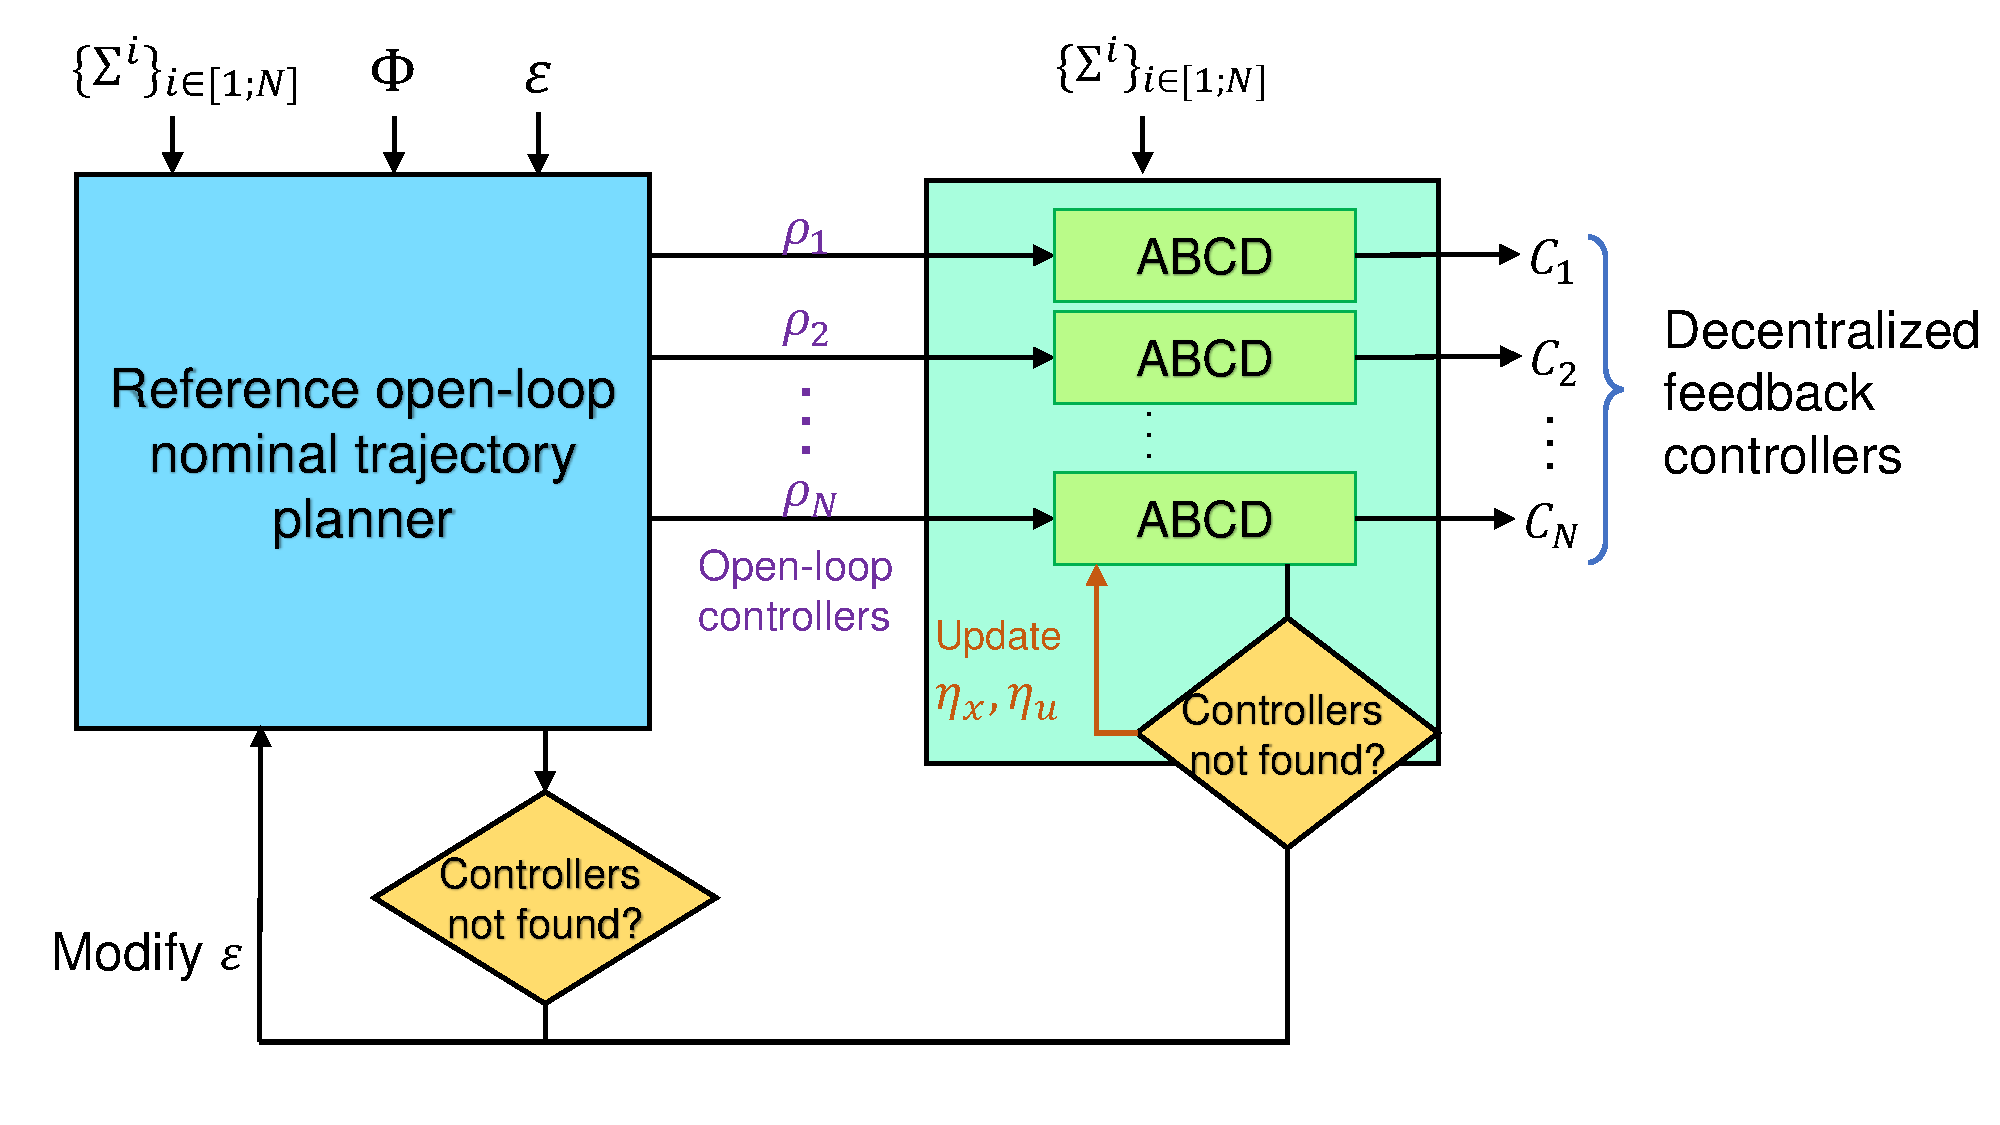
\includegraphics[width = \columnwidth]{figures/Algorithm_outline_final.pdf}
%\vspace*{-0.5cm}
\caption{Overall algorithm: The blue block on the left (centrally) computes a joint open-loop nominal trajectory for the overall system.
The green block on the right computes decentralized controllers for tracking the nominal trajectory using Abstraction Based Controller Design (ABCD).
$\Set{\Sigma^i}_{i\in [1;N]}$ is a set of $N$ agents, $\Phi$ is a global reach-avoid specification, $\varepsilon$ is a robustness margin, $\rho_1,\ldots,\rho_N$ are the local projections of the nominal trajectory, $\eta_x,\eta_u$ are parameters used in ABCD, and $C_1,\ldots,C_N$ are the sought local feedback controllers for the individual agents.
}
\label{fig:overall}
%\vspace*{-0.2cm}
\end{figure}

In this paper, we provide a simple but effective \emph{combined} approach.
We use a global planning approach for nominal trajectory generation and 
a local correct-by-construction feedback controller synthesis approach for guaranteed adherence to specification for each component
in the presence of disturbances.
Fig.~\ref{fig:overall} shows the overall algorithm.
In the first step, 
given a set of control systems, one for each component, and a reach-avoid specification on the global state space, we use a trajectory planner to
find a nominal open-loop controller for the global system.
The trajectory planner ignores the effect of disturbances, but takes a \emph{robustness parameter} $\varepsilon$.
The role of the robustness parameter is to ensure that the specification is robustly satisfied: 
Every trajectory within an $\varepsilon$-tube of the open-loop trajectory also satisfies the specification.

Next, we project the unique open-loop trajectory produced by the open-loop controller
on to a nominal trajectory for each individual component.
The robustness of the trajectory means that there is a tube around each nominal trajectory.
In a second step, we solve a number of local \emph{guaranteed tracking control} problems, where we synthesize correct-by-construction
controllers whose objective is to track the nominal trajectory while staying within the tube.
The overall algorithm is more scalable and guarantees satisfaction of the global specification.

%\KM{What does this last sentence mean? What "stronger guarantee than each component" do we provide?}
%Global trajectory planning scales to large state spaces but does not guarantee correctness and each formal controller synthesis problem is solved locally.
We show empirically that our algorithm is able to generate provably correct feedback controllers for many
systems for which neither technique is individually effective.
Of course, since we decompose the problem, it is possible that there is no controller for a particular choice of the
robustness parameter, or indeed, for other parameters used by the individual tools.
In that case, there is an outer loop that searches through the parameter space.

\begin{figure}[t]
	\centering
	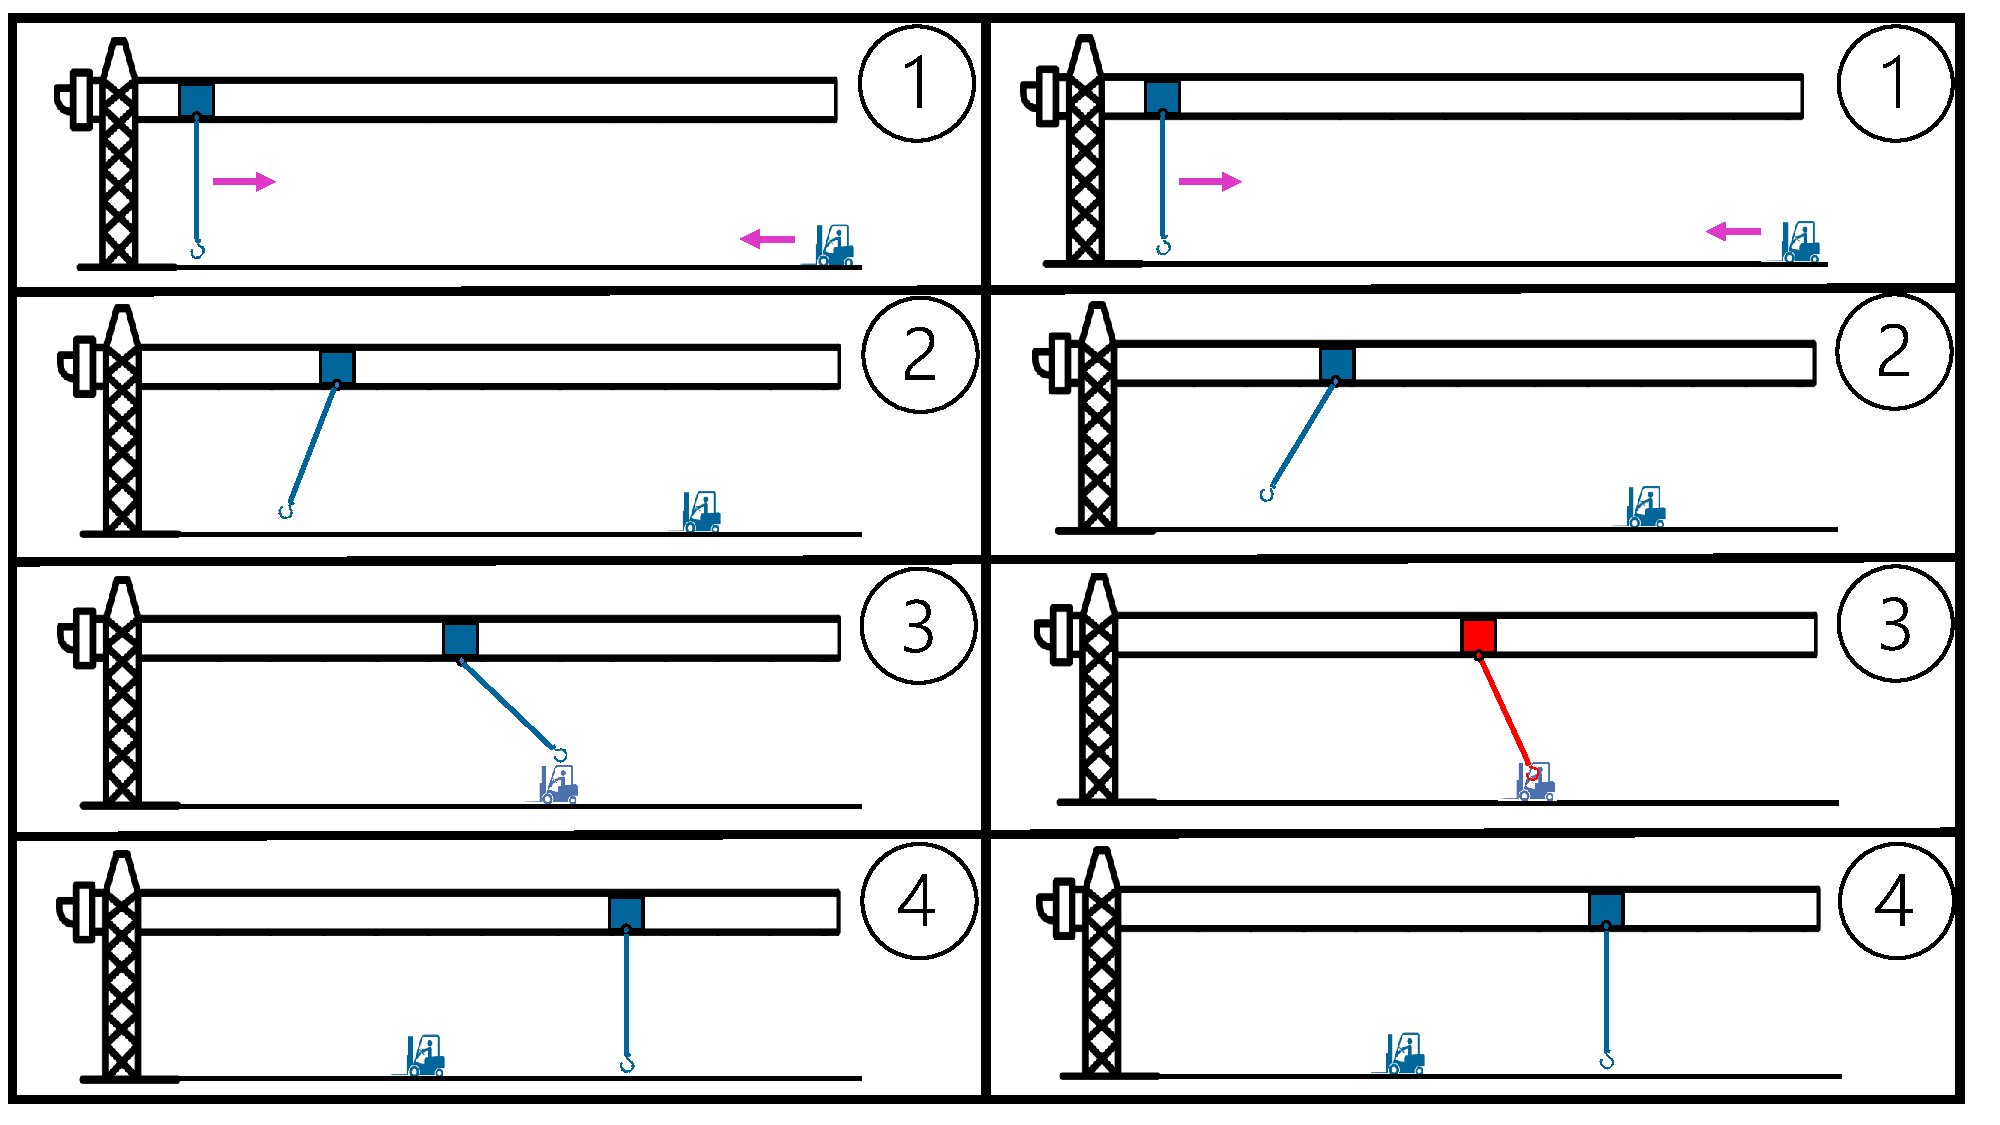
\includegraphics[width=\columnwidth]{figures/final_crane.pdf}
	\caption{Illustration of the trajectories generated by the open-loop controller for the crane and vehicle example under disturbance-free (\textbf{left}) and perturbed (\textbf{right}) situations.}
	\label{fig:cr_and_lft}
\end{figure}

We have implemented our approach in an open-source tool called \tool (stands for GuAranteed Multi-Agent Reach-Avoid control)
%\KM{Change the abbreviation if the tool name changes},
by combining the following two tools: the ALTRO open-loop trajectory planner \cite{howell2019altro} and the 
SCOTS correct-by-construction controller synthesis tool \cite{Rungger2016scots}. 
ALTRO is a state-of-the-art trajectory planning tool based on optimal control.
It handles nonlinear dynamics and scales to large dimensions, but ignores disturbances or modeling uncertainties.
SCOTS implements a highly parallelizable ABCD algorithm that generates a feedback controller for satisfying temporal specification.

We empirically evaluate \tool on a number of multi-robot benchmarks, including 
a coordinated reach-avoid problem for ground robots, 
a formation control problem for drones, and 
a lane merging schenario for autonomous vehicles.
In each case, we demonstrate that \tool can find decentralized and correct controllers within reasonable
time and memory bounds.

Fig.~\ref{fig:cr_and_lft} shows a concrete multi-robot reach-avoid scenario with an overhead crane hanging from a trolley along a horizontal rail
and a cart that drives underneath the crane in the same horizontal axis.
The goal is to move the crane and the vehicle such that they do not collide.
Fig.~\ref{fig:cr_and_lft} (\textbf{left}) shows an animation of a possible open-loop behavior from an initial configuration (Frame~1) to a final
one (Frame~4), where the crane and the vehicle have crossed each other.
The trajectory is generated by accelerating the trolley, causing the crane to swing up and thus creating enough space for the vehicle to pass.
Unfortunately, in the presence of disturbances, such as wind or a slippery floor, a trajectory may not be free of collisions: the same open-loop
behavior can cause a collision (Fig.~\ref{fig:cr_and_lft} \textbf{right}).
Instead, \tool computes a global \emph{robust} trajectory for the system; the robustness parameter ensures a ``wider berth.''
The global trajectory is projected to the crane and the vehicle, and we compute guaranteed tracking controllers that ensure there is no collision despite the disturbances.
In our experiments, planning with ALTRO took less than a second and feedback controller synthesis with SCOTS about 10 minutes.
At the same time, a global approach to find a correct solution does not scale. 
The global state space is $10^{10}$ times larger and SCOTS timed out with 1.5 TB of memory. 


 
\begin{comment}

Synthesizing formally verified controllers for safety-critical dynamical systems is an important problem. 
The goal is to \emph{algorithmically} synthesize controllers for temporal objectives
so that the closed loop systems only do what they are meant to do, even in the presence of external disturbances.




One such algorithmic technique is the so-called Abstraction-Based Controller Design (ABCD).
In ABCD, we start with a model of a continuous nonlinear dynamical system and a control task.
The sought controller is synthesized in three stages:
First, we approximate the continuous system model using a finite state abstraction.
Second, we compute an abstract controller for the abstraction by using reactive synthesis techniques.
Third, we refine the abstract controller to the sought final controller for the continuous system.
The desired correctness guarantee of the obtained controller follows from a careful abstraction construction process.

The strengths of ABCD are its versatility: 
It can handle arbitrary continuous nonlinear system models, external disturbances, modeling uncertainties, measurement errors, $\omega$-regular control specifications, and so on.
The weakness of ABCD is its poor scalability: 
Usually ABCD uses a state-space discretization for computing the abstraction, which causes an exponential blow-up in the time and space complexity.

In this paper, we extend ABCD---more in a practical sense---to synthesize controllers for a group of robots, operating in a shared workspace.
Suppose, we have a group of robots which have been assigned a joint \emph{reach-avoid} task, where the robots need to collectively reach a set of target states while collectively avoiding a set of static obstacles.
The joint task might need the robots to coordinate their actions among each other.
For example, if two robots need to jointly carry a heavy object from one place to another without letting the object fall, they need to move in perfect harmony.

Perhaps the most straightforward solution approach will be to use a centralized approach, by treating the group of robots as one single system.
In the centralized approach, we need to build a product of the models of the robots; the product captures the simultaneous evolution of the global state of the system.
Then, in theory, we can apply ABCD on the product to synthesize a global controller for the robots.
Unfortunately, the centralized approach will not be practical, because ABCD would not scale to the potentially large size of the product state space.

On the other hand, a purely decentralized synthesis, where we compute controller for each robot in isolation, is also challenging.
Usually, decentralized synthesis requires each robot to treat the other robots as adversaries, to account for the worst-case scenarios.
This is a very strong assumption, and often we will not get any controller.
For instance, recall the example of two robots jointly carrying an object.
There each of the robots will need to assume that the other robot will do everything to run away and make the object fall, which is an unrealistically strong assumption.

To circumvent these issues, in this paper, we propose a \emph{semi-centralized} and \emph{hierarchical} synthesis approach, which will give us decentralized controllers for the joint task.
In the top level, we use the centralized method with a fast synthesis tool to make a joint global plan.
In this paper, we use ALTRO \cite{howell2019altro}, which is an optimal control-based controller synthesis tool that scales quite well to large dimensional systems.
ALTRO does not provide formal guarantees against external disturbances or modeling uncertainties.
So in the bottom level, first we decompose the global plan into local plans for each robot, and then use ABCD to locally synthesize formally verified controllers to track the local plans.
(The decomposition is straightforward, because ALTRO gives us a central open-loop controller.)
Our approach is modular:
We could replace ALTRO with any other fast and scalable method, and we could replace ABCD with any other suitable method that provides guarantees, and we would still get the formally verified decentralized controllers for the robots.

We demonstrate the usefulness of our approach using several multi-robot controller synthesis examples.
\end{comment}


\begin{comment}
The collision avoidance requirement, in the absence of inter-robot communication, makes the decentralized controller synthesis problem especially challenging.
One option will be to treat the other robots as dynamic obstacles.
There are two problems.
Firstly, it is not known how to deal with dynamic obstacles in the ABCD framework.
Secondly, even if we knew how to deal with that, this dynamic obstacle assumption could lead to pessimistic, and often empty, solution.

On the other hand, the issue with dynamic obstacles goes away if we use a centralized approach, by treating the group of robots as one single system.
In the centralized approach, we need to build a product of the models of each individual robot; the product captures the simultaneous evolution of the global state of the system.
The states of collision, which are dynamic in nature, now conveniently become a set of static obstacles in the global state space.
We can then, at least in theory, use ABCD to synthesize a joint controller for the group of robots, and afterwards decompose the joint controller into individual controller for each robot.
(The decomposition is possible due to the underlying decentralized control structure.)

Unfortunately, ABCD does not scale to the usual large size of the global state space in the centralized approach.
To circumvent this issue, in this paper, we propose a two-layered hierarchical controller synthesis approach involving ABCD.
In the top layer, we use some off-the-shelf fast controller synthesis method to make a joint global plan using the aforementioned centralized approach.
In this paper, we use ALTRO \cite{howell2019altro} in the top layer, which is an optimal-control-based controller synthesis tool that scales quite well to large dimensional system.
Unfortunately, the fast and scalable tools, including ALTRO, usually do not provide formal guarantees against external disturbances or modeling uncertainties.
So in the bottom layer, we use ABCD to synthesize formally verified \emph{tracking} controller for each robot for following the projection of the joint plan on the robot's state space.
\end{comment}



\begin{comment}

\subsection{Motivating Example}

Consider a multi-robot reach-avoid problem in a factory setting:
We have an overhead crane hanging from a trolley which runs along an overhead horizontal rail; the crane is modeled as a pendulum and the trolley as an one-dimensional cart.
We also have a factory vehicle that drives underneath the crane, in the same horizontal axis as the overhead rail.
Suppose, when the crane is in the vertically downward position, it obstructs the vehicle's movement.
The scenario is illustrated in Fig.~\ref{fig:cr_and_lft} (\textbf{left}); the four different subfigures from top to bottom will be referred to as Frame~1-4 respectively.

Initially the crane is resting in its vertically downward position at the leftmost point along the rail, and the vehicle is positioned at the rightmost point (Frame~1).
Suppose in the end, they need to reach the configuration shown in Frame~4, i.e., they need to cross each other while maintaining a minimum safe distance.
To make this possible, the trolley needs to accelerate enough to swing the crane up (Frame~2-3) and create sufficient room for the vehicle to pass.
When the crane swings up high enough, the vehicle must make a timely and swift passage before the crane comes down due to gravity.
We want to design a pair of controllers, one for the trolley and one for the vehicle, which will execute this joint maneuver.

Suppose, both the vehicle and the crane are subjected to disturbances, representing (a) external factors like wind for the crane and slippery floor for the vehicle, and (b) modeling imperfections.
We want the controllers to be robust against the worst-case disturbances to the system.
In reality, worst-case disturbances might well be rare events, but safeguarding against them will certify absolute correctness.

Since we do not assume any run-time communication between the controllers, a completely decentralized synthesis would be difficult.
One option would be to assume the worst-case behavior of the other system, and attempt to achieve the goal.
This might be too restrictive:
For instance, with this assumption, the vehicle will not be able to achieve it's goal, because the crane can choose to stay down all the time.

To alleviate this issue, we employ a semi-centralized hierarchical synthesis approach.
At the \textbf{top level} of the hierarchical approach, we ignore the disturbances, and treat the crane and the vehicle as one joint system, called the \emph{product system}.
Next, we use a \emph{planner} to obtain a \emph{global} open-loop controller for the product system.
(An open-loop controller is one that bases its control decision on the current time instant.)
Among the existing off-the-shelf planning tools we selected ALTRO which is a scalable and fast controller synthesis tool that is suitable for the possibly high dimension of the product system.

Since the obtained controller is open-loop, hence we can easily decompose the central controller into individual open-loop controllers---called \emph{local} open-loop controllers---for the crane and the vehicle.
However, there will be no guarantee that the local open-loop controllers will fulfill the specification when the disturbances come into effect.
Actually, Fig.~\ref{fig:cr_and_lft}, (\textbf{left}) shows various moments in the simulation of the local open-loop controllers in the absence of the disturbances, and Frame~3 shows that the crane and vehicle get very close to each other. However, in the presence of disturbances the crane and vehicle can collide as the constraint of the minimum safe distance is violated (Fig.~\ref{fig:cr_and_lft}, (\textbf{right})). 

To deal with this robustness issue, at the \textbf{bottom level} of our hierarchical approach, we employ a \emph{guaranteed tracking method} to ``robustify'' the local open-loop controllers against disturbances.
Our choice to achieve guaranteed tracking is ABCD. More concretely, we consider the open-loop controlled trajectory of \emph{each system in isolation}, and use ABCD to synthesize a \emph{tracking controller}.
The goal of the tracking controller is to track the open-loop trajectories within some small neighborhood, even in the presence of worst-case disturbances.
ABCD gives us the sought \emph{local feedback controller} for each individual system.

\end{comment}

%\begin{figure}[t]
%	\centering
%	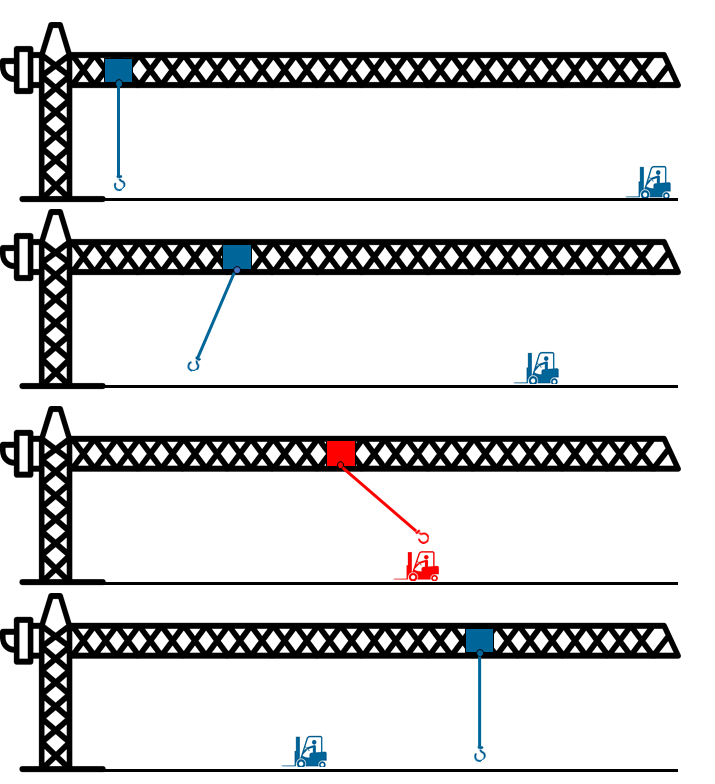
\includegraphics[width=0.45\textwidth]{figures/crane_and_lifter.png}
%	\caption{Illustration of the reference trajectories produced by the open-loop planner for the crane and the factory vehicle example}
%	\label{fig:cr_and_lft}
%\end{figure}

% !TEX root = main.tex

\smallskip
\noindent\textbf{Related Work}
%
The field of multi-agent planning is too large for a comprehensive survey; we point to the text books
\cite{LaValle2006,LaValle1998planning,choset2005principles,russel2010AIplanning} for an introduction.
We categorize closely related work into (1) the ones combining planning and tracking controller synthesis, 
(2) the ones addressing formal multi-agent controller synthesis, and 
(3) the ones combining (1) and (2). We provide a survey of these categories as follows:
%
\begin{enumerate}[(1)]
	\item Techniques combining high-level planning and low-level tracking are a staple of classical planning and control. 
More recently, several techniques consider the problem of formal guarantees for such planners.
Existing works differ in the dynamics that they can handle (e.g., linear or nonlinear),
considered class of specifications, including disturbances, and scalability. 
A common approach is to perform the high-level planning over a lower dimensional model and then use
Sum-of-Squares programming (SOS), Hamilton Jacobi (HJ), or satisfiability modulo convex programming (SMC) to obtain a low-level controller ensuring a bounded error between the 
two models \cite{herbert2017fastrack,meyer2019,singh2018robust,Nilsson:2018}. 

%\KM{Nothing has been stated about \cite{DBLP:journals/corr/abs-1911-09773,sun2019}.} 
In contrast to \cite{herbert2017fastrack,singh2018robust}, our method does not require finding 
a linear mapping between the low and high dimensional models. Meyer et al. \cite{meyer2019} considered reach-avoid problems for perturbed non-linear control affine systems. They create a lower dimensional model and use SOS programming to compute a controller ensuring a bounded error between the two models. Then, they use ABCD to compute a controller for the low-order model while taking the error into account. While their method can provide guarantee against worst-case disturbances, it is not clear if SOS always scales to the higher dimensions.

Nilsson et al. \cite{Nilsson:2018} provide a method that decomposes the state space into a lower-order planning space, and a higher-order internal dynamics space, so that fast planning and accurate tracking can be achieved using a set of control barrier functions computed based on SOS. Despite providing guarantees for the worst-case bounded disturbances, their method is not capable of solving reach-avoid tasks which involve dynamic obstacles as in the multi-agent case.
%that governs the motion in planning space. 
%The planning is performed fast since it is restricted to the lower-order space. To guarantee following of the planned trajectory in the lower-order space, control barrier functions are computed using SOS method. This method, however, cannot deal with dynamic obstacles as is needed in tackling collision avoidance.}
While we have chosen SCOTS since the underlying algorithm can be effectively parallelized \cite{KhaledZ19pfaces}, in principle, we could
also use SOS, HJ, or SMC approaches. %The existing schemes that solve the guaranteed motion planning problems in a centralized manner (e.g. \cite{sun2019}) cannot scale well.

Other works only consider special classes of models such as linear \cite{fan2018controller,wongpiromsarn2012receding,Rodionova2020LearningtoFlyLC}, 
disturbance-free \cite{tedrake2010lqr,fan2020fast,Srinivasan2018}, or finite transition systems \cite{Yang2017milp}. 
In contrast, our method supports arbitrary 
%continuous time
 nonlinear dynamics and provides a guarantee 
against worst-case bounded disturbances.
	\item Chen et al.\ \cite{Chen2018cbf} provide a method, using control barrier functions, that requires some form of inter-robot 
communication and does not consider external disturbances.
Sahin et al.\ \cite{Shahin2017cltl} propose a method that requires the group of robots to be homogeneous.
There are methods which do not consider external disturbances and do not provide formal guarantees \cite{jackson2020scalable}.
	\item Alonso-Mora et al.\ \cite{alonso2019distributed} provide a method for formation control of a group of communicating homogeneous robots.
They first synthesize nominal controller using a fast randomized geometric planning method, namely RRT, and 
then use optimal control to track the obtained nominal solution.
Unlike us, they neither consider external disturbances nor provide formal guarantees. Pant et al.\ \cite{Pant2018multiquad} have studied multi-quadrotor missions with signal temporal logic (STL) specifications. They find the reference trajectory by maximizing robustness of the STL specification, and then synthesize tracking controllers. Their method can handle only specifications with bounded horizon and does not provide guarantee against disturbances.

Recently, Xiao et al.\ \cite{xiao2019merging} propose a method for synthesis of distributed controllers for a 
set of autonomous vehicles in a lane merging situation. They consider only simple linear systems as vehicle models, use global optimal control to find a nominal controller, and employ local control barrier functions with safety constraints.
Their designed controllers is not provably safe when there is noise and can occasionally violate the safety constraints.
 %
Nikou et al.\ \cite{Nikou2019} have studied the problem of robust navigation for multi-agent systems based on nominal reference trajectory and pre-computed feedback controllers. Their approach requires sensing capabilities of the agents to avoid collision. In contrast, our method does not requires any sensing capabilities of the agents.

%They consider additive bounded modelling disturbance. 
%They use optimal control to compute a  and employ a  to keep the trajectories within a bounded distance from the reference trajectory.
Sun et al.\ \cite{sun2019} have studied motion planning of multi-agent systems with linear temporal logic (LTL) specifications, under the presence of disturbances and denial of service attacks.
Their approach uses SMC programming to compute a feasible nominal trajectory and employs feedback controllers to gain robustness.
%First, they compute a feedback controller that forces the system's trajectories to remain within a robust control invariant set under the worst-case disturbance scenario. 
%For piecewise-affine systems, there exist effective algorithms for computing the feedback controller and the corresponding invariant set. 
%Next, they use  together with an open-loop controller, and by adding up the nominal open-loop control input and the feedback control law they construct the final control input.
Despite being able to provide guarantees against disturbances, their implementation is centralized, thus the required time increases significantly for high-dimensional reach-avoid specifications.%The main drawback of their method is central implementation, since tackling reach-avoid problems in higher dimensions takes significantly longer time.
 %However, they assume that agents are able to communicate while moving; and their target is to satisfy input-to-state stability. In fact, their method is not able to tackle collision avoidance for static/dynamic obstacles.}
%
There are other works that use a pre-defined motion primitive library to perform planning for multi-robot 
systems \cite{saha2016implan,BanusicMPSZ19pgcd,Gavran2017antlab,desai2017drona}. 
In contrast, our method deals with the dynamical model directly.

Our construction can also be seen as an \emph{assume-guarantee} technique that decomposes the global problem based on nominal trajectory tubes. Similar decompositions have been studied in the discrete case \cite{alur2015pattern,majumdarassume}.
The closest related work that matches our level of generality is the work by Bansal et al.\ \cite{bansal2017safe}.
However, they assume that each robot has its own reach-avoid specification while avoiding collision with the other robots.
In contrast, we allow global reach-avoid specifications, which subsume their class of specifications.
In fact, there are control problems that can be easily handled by our approach and cannot be encoded in their setting. An example is robots maintaining a formation while fulfilling their tasks \cite{alonso2019distributed}.
\end{enumerate}

%Our experiments show that \tool is efficient in solving reach-avoid tasks for multi-agent systems. 
%However, there are other tools which claim they can solve similar tasks. 
A subset of approaches listed above have available implementations.
In Table~\ref{tab:tools}, we summarize the main features of the publicly available tools.
We highlight that our tool \tool is the only one that fulfills all the criteria.

\begin{table}
	\large
	\centering
	\caption{Features of the publicly available tools compared to \tool. Note that some of these tools can handle richer classes of specifications, compared to the reach-avoid problem handled by \tool.}\label{tab:tools}
	\renewcommand{\arraystretch}{1.2}
	\setlength{\tabcolsep}{0.7em} % for the horizontal padding
	%\resizebox{1\columnwidth}{!}{
	\begin{tabular}{l 
							>{\centering}m{5mm}
							>{\centering}m{5mm} 
							>{\centering}m{5mm}	
							>{\centering\arraybackslash}m{5mm}}
		\toprule
		Tool name &
		\rotatebox{90}{Non-linear Dynamics} & \rotatebox{90}{Formal Guarantee} & \rotatebox{90}{Multi-agent} & \rotatebox{90}{Decentralized controllers}\\
		\hline
		\rowcolor{black!20} \tool  & \ding{51} &\ding{51} & \ding{51} &  \ding{51}\\
		\hline
		SCOTS \cite{Rungger2016scots}	&	\ding{51}	&	\ding{51}		&		&	\\
		\hline
		ALTRO \cite{howell2019altro}		&	\ding{51}	&	&	&\\
		\hline
		FastTrack \cite{herbert2017fastrack}& \ding{51} & \ding{51} &   &   \\
		\hline
		RealSyn \cite{fan2018controller}& &\ding{51} &  &  \\
		\hline
		Factest \cite{fan2020fast}& \ding{51} &  &  &  \\
		\hline
		Model mismatch (SOS) \cite{singh2018robust}  & \ding{51} &  &  &  \\
		\hline
		RTD \cite{kousik2020bridging} & \ding{51} & \ding{51} &  &  \\
		\hline
		Fly-by-Logic \cite{Pant2018multiquad}  & \ding{51} & & \ding{51} & \ding{51} \\
		\hline
		Distributed team lift \cite{jackson2020scalable} & \ding{51} &  & \ding{51} &  \\
		\bottomrule
	\end{tabular}
\end{table}

	%The hierarchical approach, combining high-level planning and low-level tracking, is not new.
	%Yet most of the existing works use the hierarchical approach for controller synthesis for a single robot \cite{herbert2017fastrack, fan2020fast, fan2018controller, wongpiromsarn2012receding, tedrake2010lqr, singh2018robust, DBLP:journals/tac/MeyerD19, DBLP:journals/corr/abs-1911-09773, Yang2017milp}.
	%In contrast, we consider a hierarchical control for decentralized control of a group of robots.
%	For example, there are methods which can generate nominal controlled trajectories by taking into account the maximum tracking error, assuming that a tracking controller is already in place \cite{fan2020fast, fan2018controller}.
%	On the other hand, there are methods which compute a tracking controller which minimizes the tracking error for any given nominal trajectory:
%	Some of them do not consider external disturbances \cite{tedrake2010lqr, singh2018robust}, some of them only consider linear dynamics \cite{wongpiromsarn2012receding}, and all of them consider only a single monolithic system structure \cite{herbert2017fastrack}.

% Many papers address the problem of multi-robot controller synthesis without a hierarchical approach.


% In contrast, our method can synthesize formally verified controllers for heterogeneous group of robots, subjected 
% to external disturbances, and lacking any form of communications. 
% Hierarchical controller synthesis for decentralized control of multi-robot systems is relatively rare.

% In contrast, our method provides guarantee against worst-case system noise at all time, and in addition can support nonlinear systems. 
 

%\begin{enumerate}
%	\item FastTrack: Guaranteed tracking of nonlinear trajectories for nonlinear systems under disturbances \cite{herbert2017fastrack}. \MS{They only account for the error between the planning and tracking models and not for additive disturbance applied to the tracking model. They also rely on possibility of relating the two afformentioned models by a linear mapping (which is not the case for the general class of systems). Finally, while their method scales up better than (pure) SCOTS, it does not scale up to dimensions above ten.}
%%	\item Using the tracking error in the planning phase to make sure that the controller will be safe \cite{fan2020fast}. Relies on an expert user to already provide the low-level tracking controller, whereas we synthesize the tracking controller. So they address the inverse problem in some sense.
%%	\item Another paper of the same flavor as the previous one \cite{fan2018controller}. Here they restrict themselves to discrete time perturbed linear systems.
%%	\item Sum-of-squares based tracking methods \cite{tedrake2010lqr, singh2018robust}. Do not consider external disturbances.
%	\item Other hierarchical methods using planning+tracking like approach for formal methods-based synthesis for single systems \cite{wongpiromsarn2012receding, DBLP:journals/tac/MeyerD19, DBLP:journals/corr/abs-1911-09773}.
%	
%	\item A robust scheme for controlling linear dynamical systems with additive bounded noise and (general) LTL specification \cite{Yang2017milp}. They use mixed integer linear programming (MILP) to design a nominal controller satisfying a given LTL specification in the absence of noise and then design a regulating controller to account for the noise term.
%\end{enumerate}

%\smallskip
%\noindent\textbf{Ones which address multi-robot control problems.}\
%
%\KM{The plan is to collect all the papers first in the following list. After that, I will make a story out of them.}
%Here are the papers that we know of:
%\begin{enumerate}
%	\item Safe control for multi-vehicle system under presence of disturbances \cite{bansal2017safe}. In contrast to our method, they assume a fixed priority order of the vehicles: The higher priority vehicles make independent plans, which are treated as (time-varying) obstacles for the lower priority vehicles. 
%	\new{One way our method is probably more powerful is if we consider controller synthesis for mechanically coupled systems with joint goal, or even formation control problem for mechanically decoupled systems. For these class of problems, I don't think their method will directly apply, whereas ours should work fine.}
%	
%	\item A method to control a robot swarm (modelled as planar robots with potentially different speed bounds) such that a given specification (expressable in a fragment of LTL) is satisfied \cite{Chen2018cbf}. Some extent of communication between robots is required. The collision avoidance is guaranteed via designing control barrier functions for each pair of robots. No source of disturbance is considered in the model and the proposed solution does not work for agents modeled not as planar robots.
%	\item Controlling (homogeneous) robot swarms (modelled as finite state transition systems) for satisfying specifications expressed in a temporal logic for reasoning about the collective behavior of multiple agents (cLTL) \cite{Shahin2017cltl}. Their method can potantially account for bounded noise and non-linearities, but not heterogeneity.
%	\item Controlling multi-robot (it can be heterogeneous) using ALTRO \cite{jackson2020scalable}. very similar to our work without formal guarantee but works in real-time. they are making centralized system by combining dynamics of several quads. 
%	\item The paper that we got merging example from that\cite{xiao2019merging}. They are using optimal control + control barrier function. they are can handle disturbance and in addition they are optimizing time and fuel consummation and more constraints but they are considering linear model.
%	\item Hierarchical control for interconnected discrete event systems \cite{wong1996hierarchical,schmidt2008nonblocking}.
% \end{enumerate}

%! TEX ROOT = ./main.tex

\section{Preliminaries}

\smallskip
\noindent\textbf{Notation.}\
We use the notation $\mathbb{R}$ and $\mathbb{R}_{>0}$ to denote the set of real numbers and the set of positive real numbers respectively.
We use superscript $n>0$ with $\mathbb{R}$ and $\mathbb{R}_{>0}$ to denote the cartesian product of $n$ copies of $\mathbb{R}$ and $\mathbb{R}_{>0}$ respectively.
Given two points $x=(x_1,\ldots, x_n)$ and $y=(y_1,\ldots, y_n)$ in $ \mathbb{R}^n$ (or $\mathbb{R}^n_{>0}$) and a relational symbol $\triangleright\in \set{\leq, <, = , >, \geq}$, we write $x\triangleright y$ if for every $i=1,\ldots,n$, $x_i\triangleright y_i$.
The operator $|\cdot |$ is used to denote both the absolute value of a vector and cardinality of a set, depending on the type of the operand, and the operator $\| \cdot \|$ is used to denote the infinity norm.  

Let $f\colon A\to B$ and $g\colon C\to D$ be two functions.
We define the product function $f\otimes g\colon A\times C\to B\times D $, $f\otimes g \colon (a,c)\mapsto (f(a),g(c))$.
The product function can be defined for arbitrarily many functions by extending the definition in the obvious way.

%Throughout, we measure distance between two points, within a space $\mathbb{R}^n$, using the \emph{distance metric} $d\colon \mathbb{R}^p\times \mathbb{R}^p\to \mathbb{R}_{\geq0}$, $d^p\colon \left(u,v\right)\mapsto \|u-v\|$. 
%We extend the definition of $d^p$ to measure distance between a point and a set: for any given $u\in \mathbb{R}^p$ and $V\in \mathbb{R}^p$, $d^p(u,V) \coloneqq \inf_{v\in V}\|u-v\|$.
Given a point $c\in \mathbb{R}^n$ and given the parameter $\varepsilon\in \mathbb{R}_{>0}^{n}$, we use the notation $\ball_\epsilon( x)$ to denote the ball in $\mathbb{R}^n$, centered around $c$ and having radius $\epsilon$.
Formally, \[\ball_\varepsilon(c)\coloneqq \set{x
	\in \mathbb{R}^n \mid  |x-c|\leq \varepsilon }.\] 

Let $A$ be a set.
We use the notation $A^\infty$ to denote the set of all finite and infinite sequences formed using the members of $A$. Finally, to define our control tasks, we use a subset of Linear Temporal Logic (LTL). In particular, we will use the until ($\mathcal{U}$) and next  ($\bigcirc$) operators. In brief, For detailed syntax and semantics of LTL, we refer to \cite{baier2008principles} and references therein.

%Let $V$ be a finite set of real-valued variables.
%We use the notation $\sem{V}$ (same symbol but in boldface blue) to denote the set of every possible valuations of the variables in $V$, i.e.\ an element in $\sem{V}$ assigns an unique real number to every variable in $V$.
%It is easy to see that $\sem{V} = \mathbb{R}^{|V|}$.
%Let $U\subset V$ be a set.
%For any $v\in \sem{V}$, we use the notation $v[U]$ to denote the valuation in $\sem{U}$ that assigns the same values to the variables in $U$ as assigned by $v$; $v[U]$ is called the projection of $v$ on to $U$.

%Let $V$ be a finite set of real-valued variables, as above.
%Given any two points $u,v\in \sem{V}$ with $u=(u_1,\ldots,u_{|V|})$ and $v=(v_1,\ldots,v_{|V|})$, we introduce the \emph{element-wise distance function} $d_V\colon \sem{V}\times \sem{V}\to \mathbb{R}^{|V|}_{>0} $, $d_V\colon (x,y) \mapsto (|x_1-y_1|,\ldots, |x_{|V|}-y_{|V|}|)$.
%We sometime exploit the notation and use the same $d_V$ to measure the distance between a set $W\subseteq \sem{V}$ and a point $v\in \sem{V}$, which is defined as follows:
%$d_V(v,W)= (\inf_{w\in W} |v_1-w_1|, \ldots, \inf_{w\in W} |v_{|V|}-w_{|V|}|)$.

\subsection{System Formalisms}
 
\smallskip
\noindent\textbf{Control System.}\
A \emph{control system} $\Sigma = (X, x_{\init}, U, W, f)$
consists of a \emph{state space} $X\subseteq \mathbb{R}^n$,
an \emph{initial state} $x_\init\in X$,
 an \emph{input space} $U\subseteq\mathbb{R}^m$, 
a compact \emph{disturbance set} $W\subset \mathbb{R}^n$ and
a \emph{nominal dynamics} $f:X\times U\rightarrow X$ such that $f(\cdot,u)$ is locally Lipschitz for all $u\in U$.%, an \emph{output space} $Y\subseteq \mathbb{R}^p$, and
%an \emph{output function} $h\colon X\mapsto Y$. 
%
%We call each element of the set $\sem{X}$ a \emph{state}, and the set $\sem{X} = \mathbb{R}^{|X|}$ the \emph{state space} of $\Sigma$.
%Throughout, we will assume that there is a metric $d\colon \sem{X}\times \sem{X}\to \mathbb{R}$ on the set $\sem{X}$ such that $(\sem{X},d)$ is a metric space. 

Given a time horizon $T>0$, and a constant input $u\in U$, 
a (state) \emph{trajectory} of $\Sigma$ 
on $[0,T]$ is an absolutely continuous function $\xi:[0,T]\rightarrow X$  such that $\xi(0) = x_\init$ and
$\xi(\cdot)$ fulfills the following differential inclusion for almost every $t\in[0,T]$:
\begin{equation}\label{equ:def_f}
 \dot{\xi}\in f(\xi(t),u) + W. 
\end{equation} 
We collect all such solutions in the set $\Sol_\Sigma(x_0,u,T)$. 

\smallskip
\noindent\textbf{Transition System.}\
A \emph{state-transition system} $S=(Z,z_\init,U,\delta)$ consists of a \emph{state space} $Z$, an \emph{initial state} $z_\init\in Z$, an \emph{input space} $U$, and a \emph{transition function} $\delta:Z\times U \rightarrow 2^Z$. 
A system $S$ is \emph{finite} if $Z$ and $U$ are finite. 
A \emph{trajectory} of $S$ is a maximal sequence of states $\rho = (z_0,z_1,\ldots) \in Z^\infty$ starting at $z_0=z_\init$ and compatible with $\delta$:
for all $1\leq k < |\rho|$ there exists $u\in U$ such that $z_k\in \delta(z_{k-1},u)$ and 
if $|\rho| < \infty$ then $\delta(z_{|\rho|},u)= \emptyset$ for all $u\in U$.
%For $D\subseteq X$, a $D$-trajectory is a trajectory $\xi$ with $\xi(0)\in D$.

%\subsection{System Composition}

\smallskip
\noindent\textbf{Product Control System.}\
Let $\set{\Sigma^i}_{i\in [1;N]}$, $\Sigma^i=(X^i,x_\init^i,U^i,W^i,f^i)$, be a set of $N$ control systems. 
We assume that all of the control systems within $\set{\Sigma^i}_{i\in [1;N]}$ share an output space $Y\subseteq\reals^p$ to which there exists a set of projections of the form $h^i\colon X^i\rightarrow Y$. Remember our motivating example, wherein the crane's state space contains the cart's position ($z$), the cart's speed ($\dot z$), the pendulum's angular position ($\theta$) and speed ($\dot \theta$). The state space for the forklift is described with only one state variable $z'$ describing its position. Note that $X^1\subseteq \reals^4$ and $X^2\subseteq \reals$. Now, defining $h^1=\begin{bmatrix}z+l\sin(\theta)&y_1+l\cos(\theta)\end{bmatrix}^T$ and $h^2=\begin{bmatrix}z'&y_2\end{bmatrix}^T$, both state spaces can be projected to $Y\subseteq \reals^2$ in which we would like to compute distance.
%For example, in a multi-robot scenario, all of the robots move within a two or three dimensional space independent of their individual dynamics.
We define distance between two control systems as $D\colon X^i\times X^j\rightarrow \reals_{\geq 0}$, $D\colon (u,v)\mapsto\| h^i(u)-h^j(v)\|$. We extend the definition of $D$ to measure distance between a system's state and a set defined over the shared output space: for any given $u\in X^i$ and $V\subseteq X^i$, $D(u,V) \coloneqq \inf_{v\in V}\|u-v\|$. The \emph{product control system of } $\set{\Sigma^i}_{i\in [1;N]}$ is the control system $\Sigma^\times = (X^\times, x_\init^\times, U^\times, \set{0^n}, f^\times, D)$ wherein $X^\times\coloneqq X^1\times \ldots \times X^N$ and we assume that $\sum_{i\in [1;N]} n_i=n$, $x_\init^\times\coloneqq (x_\init^1,\ldots,x_\init^N)$, $U^\times\coloneqq U^1\times\dots\times U^N\subset \reals^m$ and $f^\times\coloneqq f^{1}\otimes \ldots\otimes f^{N}$. 
We use the state projection operator $\proj^{i}\colon X^\times\to X^i$, $\proj^{i}\colon (x^1,\ldots,x^N)\mapsto x^i$.
From here on, we will omit the domain of $i$ and will use ``$\set{\Sigma^i}$'' instead of ``$\set{\Sigma^i}_{i\in [1;N]}$'' for simpler notation.

\smallskip
\noindent\textbf{Product Transition System.}\
Let $\set{S^i}_{i\in [1;N]}$, $S^i=(Z^i,z_\init^i,U^i,\delta^i)$, be a set of $N$ transition systems.
The \emph{product transition system of } $\set{S^i}_{i\in [1;N]}$ is the transition system $S^\times \coloneqq (Z^\times, z^\times, U^\times, \delta^\times)$ such that $Z^\times \coloneqq Z^1\times \ldots \times Z^N$, $z^\times_\init\coloneqq (z_\init^1,\ldots,z_\init^N)$, $U^\times \coloneqq U^1\times \ldots\times U^N$, and $\delta^\times \coloneqq \delta^1\otimes\ldots \otimes \delta^N$.
From here on, we will omit the domain of $i$ and will use ``$\set{S^i}$'' instead of ``$\set{S^i}_{i\in [1;N]}$'' for simpler notation.

\subsection{Controllers} Here, we only introduce the notations for representing different types of controllers used in this paper. More detailes can be found in Sec.~\ref{sec:controllers}. Let $\Sigma_\tau=(X,x_\init,U,f_\tau)$ denote sampled time abstraction of a control system $\Sigma$ for a given sample time $\tau>0$. An open-loop controller of $\Sigma_\tau$ is a function $C\colon [0;T]\to U$ for some given time horizon $T>0$. The open-loop is obtained when we connect $C$ with $\Sigma_\tau$ serially (denoted by $C \triangleright \Sigma_\tau$). The \emph{open-loop behavior} $\Beh^\ol(x_\init)$ of $\Sigma_\tau$ under $C$ is the set of all trajectories of the transition system $C \triangleright \Sigma_\tau$. A feedback controller of $\Sigma_\tau$ is a function $C\colon X\to U$. The closed-loop is obtained when we connect $C$ with $\Sigma_\tau$ in feedback (denoted by $C\parallel\Sigma_\tau$). %The \emph{closed-loop behavior} $\Beh^\cl(x_\init)$ of $\Sigma_\tau$ under $C$ is the set of all trajectories of the transition system $C\parallel\Sigma_\tau$. 
Let $\Sigma^\times_\tau$ be the product sampled time abstraction of $\set{\Sigma^i} $.
A global open-loop (feedback) controller of $\set{\Sigma^i} $ is an open-loop (a feedback) controller of $\Sigma_\tau^\times$.
On the other hand, a set of local open-loop (feedback) controllers of $\set{\Sigma^i_\tau} $ is a set $\set{C^i} $ where, for every $i\in [1;N]$, $C^i$ is an open-loop (a feedback) controller of $\Sigma^i_\tau$.

%here
%\subsection{Abstraction-Based Controller Synthesis Background}
%Let $\Sigma = (X, U, W, f, \cdot, \cdot)$ be a control system, $\tau>0$ be the sampling time, $\bound$ be a subset of $X$ which imposes a safety specification, $\Xh$ be a given \emph{finite partition} of $\bound$, and $\Uh$ be a \emph{finite subset} of equally spaced (w.r.t.\ infinity norm on $\mathbb{R}^m$) points in the set $U$. A \emph{finite-state abstraction} of $\Sigma$ is a finite state-transition system $(\Xh,\Uh,\fh)$, where $\xh'$ is in $\fh(\xh,u)$ if there is a pair of states $x\in \xh$ and $x'\in \xh'$ such that there is a trajectory $\xi\in \Sol_\Sigma(x,u,\tau)$ with $\xi(\tau)=x'$.
%
%We assume that the size of the partition elements is provided as a vector $\eta_x\in \mathbb{R}^n_{>0}$ which is an input to the abstraction procedure. We also assume that the set $\Uh$ is chosen based on an input-space discretization parameter $\eta_u\in \mathbb{R}^m_{>0}$. 
%
%We assume that there is a black-box procedure named $\findAbs$ which takes as input the description of $\Sigma = (X,U,W,f,\cdot,\cdot)$, a compact subset $\bound$ of the set $X$, a sampling time $\tau>0$, and state space and input space discretization parameters $\eta_x$ and $\eta_u$ respectively, and returns a finite-state abstraction $\widehat{\Sigma} = (\Xh,\Uh,\fh)$ of $\Sigma$ and a feedback refinement relation $Q$ from $\Sigma_\tau$ to $\hat\Sigma$. More details can be found in Sec.~\ref{sec:abcd}.
%here
%! TEX ROOT = ./main.tex

\section{The Problem Statement}
%\textcolor{blue}{
In this paper, we consider the planning problem for a heterogeneous swarm of $N$ robots under the presence of external disturbances and model uncertainties. 
The robots' nominal dynamics can be non-linear and there can be bounded noise in the model, capturing the effect of the disturbances and model uncertainties.
We further assume that the robots are incapable of synchronizing their actions through communication among each other during run-time.
We want to synthesize individual feedback controllers for every robot so that the following conditions are fulfilled:
\begin{description}
	\item[Reachability:] Every robot, when positioned at a designated initial state, should eventually reach a designated target state.
	\item[Obstacle avoidance:] No robot should collide with the given set of static obstacles.
	\item[Collision avoidance:] No two robots should ever collide against each other.
\end{description}
For the sake of simplicity, at the controller synthesis stage, we ignore the geometry of the robots and model them as point masses.
Then the collision avoidance requirement is formalized by requiring the robots to maintain certain minimum distance from every other robot, as if there is a bounding box around each point mass robot and we require that no two bounding boxes should ever come in contact with each other.

%\textcolor{blue}{%We consider planning problem for multi-robot systems modelled collectively as control system $\Sigma$ with order $n=\sum_{i=1}^N n_i$. Each of $N$ robots can be represented as a control system of order $n_i$ 
We fomalize the problem statement in the following.
We start with the following six ingredients that are required to be provided as inputs:
\begin{description}
	\item[System model:] Every robot is modeled as a control system $\Sigma^i = (X^i, U^i, W^i, f^i)$ for $i\in [1;N]$. 
	We assume that there is a set of \emph{global state variables} $Z$ such that for every $i\in [1;N]$, $Z\subseteq X^i$.
	For every $\Sigma^i$, every state variable that is not global is called a \emph{local state variable}.
	We assume that the set of local state variables of all the systems are pairwise disjoint. 
	\item[Sampling time:] A sampling time $\tau\in \mathbb{R}_{>0}$.
	\item[Initial states:] Every robot has a designated initial state $\init^i\in \sem{X^i}$ for $i\in [1;N]$.
	\item[Target states:] Every robot has a designated set of goal states $\goal^i\subseteq \sem{X^i}$  for $i\in [1;N]$.
	\item[Static obstacles:] Every robot has a, possibly empty, set of static obstacles $\obs^i\subseteq \sem{X^i}$  for $i\in [1;N]$.
%	\item[Global (static) obstacles:] A, possibly empty, set of global static obstacles $\avoidg\subseteq \sem{Z}$.
	\item[Safety margins:] A collision margin $\delta_{\col}\in \mathbb{R}^{|Z|}_{>0}$ which denotes the required minimum distance between every two robots, and a set of obstacle margins $\set{\delta_{\obs,i}}_{i\in [1;N]}$, with $\delta_{\obs,i}\in \mathbb{R}^{|Z|}_{>0}$ for all $i$, which denote the required minimum distance between every robot and the obstacles.
\end{description}

A set of feedback controllers $\set{C^i}_{i\in [1;N]}$ for the systems $\set{\Sigma_\tau^i}_{i\in [1;N]}$ \emph{realizes} the given specification $(\set{\init^i}_{i\in [1;N]}, \set{\goal^i}_{i\in [1;N]}, \set{\obs^i}_{i\in [1;N]}, \delta_\col, \set{\delta_{\obs,i}}_{i\in [1;N]})$, as defined above, if the following conditions are satisfied:
For \emph{every} $i\in [1;N]$ and for \emph{every} infinite behavior $(x_0^i,x_1^i,\ldots)\in \Beh^\cl(x_0^i)$ of the closed loop $C^i\parallel \Sigma_\tau^i$ starting at $x_0^i=\init^i$, there \emph{exists} a $K$ such that
\begin{description}
	\item[Reachability:] $x_K^i\in \goal^i$.
	\item[Obstacle avoidance:] For every $k\leq K$, we have $d_{X_i}(x_k^i,\obs^i) > \delta_{\obs,i}$.
	\item[Collision avoidance:] 
		Suppose $j\in [1;N]$ with $j\neq i$ be some other system index.
		Consider any arbitrary infinite behavior $(x_o^j, x_1^j,\ldots)\in \Beh^\cl(x_0^j)$ of $C^j\parallel \Sigma_\tau^j$ starting at $x_0^j=\init^j$. 
		Then for every $k\leq K$ we require the following to be satisfied: $d_{Z}(x^i_k[Z],x^j_k[Z])>\delta_{\col}$.
\end{description}

\begin{comment} % Mahmoud's version
\KM{I am not sure if the highlighted text below is used anywhere so far.}
\new{
We define the \emph{product control system} $\Sigma = (X, U, W, f)$ wherein $X=X^1\times X^2\times\dots\times X^N=\reals^n$, $U=U^1\times\dots\times U^N\subset \reals^m$, $W=W^1\times\dots\times W^N\subset \reals^n$ and $f=f^{1}\oplus \ldots\oplus f^{N}$. 
Intuitively, the product control system models the joint behavior of the robotic swarm.
}
We consider a setting wherein each individual robot starts from a (known) initial state $x_0^i\in X^i$ and is asked to go into a \emph{neighborhood} of its corresponding goal state $x_G^i\in X^i$ under the presence of non-zero disturbance. Concatenated initial and goal states of the collective swarm robot system are denoted by $x_0=\begin{bmatrix}{x_0^{1^T},\ldots,x_0^{N^T}}\end{bmatrix}$ and $x_G=\begin{bmatrix}{x_G^{1^T},\ldots,x_G^{N^T}}\end{bmatrix}$.
We denote by $\obs$ the set of polytopic (static) obstacles scattered in $\reals^2$ and by $\reach\subset X$ for the targetted neighborhood of the collective system.%}

%We consider a setting wherein each individual robot starts from a (known) initial state $x_0^i$ and is asked to go into a \emph{neighborhood} of its corresponding goal state $x_G^i$. We denote by $\obs$ the set of polytopic (static) obstacles scattered in $\reals^2$. %For a given control system $\widetilde\Sigma$, the targetted problem is denoted by a tuple $(\reach,obs,x_0)$, where $x_0\in X$ is a designated initial state, and $\reach$ and $obs$ are subsets of the state spaces $X$.
 %Any collision avoidance scheme ensures that minimum distance between robots is always greater than By (static) obstacle $\avoid$ is selected so that it consists a neighbour
For a given sampling time $\tau>0$ and positive constants $\delta_{\col}$ and $\delta_{\obs}$, a feedback controller $C$ \emph{realizes} the desired specification on $\Sigma_\tau$ if the closed-loop behavior $\Beh^\cl(x_0)$ of $C\parallel\Sigma_\tau$ satisfies the following condition: For \emph{every} infinite sequence $(x_0,x_1,\ldots)$ in $\Beh^\cl(x_0)$,
\begin{itemize}
 \item there \emph{exists} a $K$ s.t.\ $x_K\in \reach$ 
 
 \item for \emph{every} $k\leq K$ and every $1\leq i,j \leq N$ we have $d(x^i_k,x^j_k)>\delta_{\col}$ for $i\neq j$, and
 
 \item for \emph{every} $k\leq K$ and every $1\leq i\le N$ we have $D(x^i_k,obs)>\delta_{\obs}$.
 
 \end{itemize}
 %We denote by $\avoid$ the subset of state-time space at which the second condition above does not hold.
 For a given control system $\Sigma$, the targetted problem is denoted by a tuple $(x_0, \reach,\obs, \delta_{\obs},\delta_{\col})$. In linear temporal logic (LTL) notation \cite{baier2008principles}, the above conditions can be succinctly written as:
\begin{equation}\label{eq:spec}
	x_0 \wedge ([\bigwedge_{1\leq i\leq N}D(x^i,\obs)>\delta_{obs}\; \bigwedge_{1\leq i,j\leq N\;i\neq j}  d(x^i,x^j)>\delta_{\col}]\; \mathcal{U}\;\reach) .
\end{equation}
\end{comment}

\begin{problem}\label{prob:reach-avoid}
	Given a set of control systems $\set{\Sigma^i}_{i\in [1;N}$, a sampling time $\tau\in \mathbb{R}_{>0}$, and a specification $(\set{\init^i}_{i\in [1;N]}, \set{\goal^i}_{i\in [1;N]}, \set{\obs^i}_{i\in [1;N]}, \delta_\col, \set{\delta_{\obs,i}}_{i\in [1;N]})$, find a set of feedback controllers $\set{C_i}_{i\in [1;N]}$ for the systems $\set{\Sigma_\tau^i}_{i\in [1;N]}$ which realize the given specification.
\end{problem}

%\KM{An weird thing I noted is that the systems cannot violate their "local" obstacle avoidance specification until all the systems have reached their targets. This is stronger than a simple "until" type local specification for each robot, where it is required that the obstacles are not hit before reaching the target for the first time. This is just an observation: nothing breaks.} \MZ{"This point is needed to be discussed"}

We categorize the available controller synthesis techniques from the existing literature into two broad groups, namely the $\mathit{fast}$ ones and the $\mathit{sound}$ ones.
The $\mathit{fast}$ ones are those which are extremely efficient, but do not provide formal worst-case robustness guarantee of the controller against external disturbances \cite{howell2019altro,choset2005principles}.
The $\mathit{sound}$ ones are those which are not so efficient, but provide strong formal guarantee on the correctness of the controller \cite{reissig2016feedback,fisac2015reach,tedrake2009lqr}.
%In Sec.~\ref{sec:nominal trajectory} and Sec.~\ref{sec:tracking}, we propose a hierarchical solution approach for Prob.~\ref{prob:reach-avoid} that marries the $\mathit{fast}$ and the $\mathit{sound}$ solution techniques.

We propose a hierarchical solution approach for Prob.~\ref{prob:reach-avoid} that marries the $\mathit{fast}$ and the $\mathit{sound}$ solution techniques.
Our approach is a two-stage procedure: 
\begin{itemize}
	\item First, we deploy an off-the-shelf $\mathit{fast}$ method to quickly solve the controller synthesis problem, and obtain a set of  \emph{valid} (controlled) \emph{nominal trajectories} $\set{(x_{0_\nom}^i,\ldots,x_{K_\nom}^i)}_{i\in [1;N]}$, for the systems $\set{\Sigma_\tau^i}_{i\in [1;N]}$, such that the following conditions are met:
	\begin{itemize}
		\item For every $i\in [1;N]$, there exists $k\in [0;K]$, such that $x_{k_\nom}^i\in \goal^i$,
		\item for every $i\in [1;N]$ and for every $k\in [0;K]$, $d_{X_i}(x_{k_\nom}^i,\obs^i) > \delta_{\obs,i}$, and
		\item for every $(i,j)\in [1;N]\times [1;N]$ and for every $k\in [0;K]$, $d_{Z}(x_{k_\nom}^i[X^i\cap Z], x_{k_\nom}^j[X^j\cap Z]) > \delta_\col$. 
	\end{itemize}
	(Essentially, a set of valid nominal trajectories is a witness trajectory for the satisfaction of the specification.)
	While, in principle, any $\mathit{fast}$ method could be used for this first phase, in this work we solve the given problem \emph{centrally} using the tool called ALTRO \cite{howell2019altro}.
	\item Second, for every $\Sigma^i_\tau$, for $i\in [1;N]$, we use a $\mathit{sound}$ method to compute a sound feedback controller which \emph{tracks} the respective nominal trajectory of system $\Sigma^i_\tau$ up to a given precision.
The main contribution of this paper is an efficient implementation of this second stage, which is formalized as a separate problem in the following:
		\begin{problem}\label{prob:tracking_with_time}
			Let $\Sigma=(X,U,W,f)$ be a control system, $\tau>0$ be a sampling time, $\goal\subseteq \sem{X}$ be a designated target set, $(x_{0_\nom},\ldots,x_{K_\nom})$ be a given finite nominal trajectory, and $\varepsilon\in \mathbb{R}^{|X|}_{>0}$ be a precision parameter chosen in such a way that there exists a state $g\in \goal$ such that the following holds:
			\begin{equation}\label{eq:choice of eps}
				\varepsilon \leq d_X(g, \sem{X}\setminus \goal). 
			\end{equation}
			Find a feedback controller $C$ for $\Sigma_\tau$ such that 
			% for every initial state $x_0\in X$ with $\| x_0-x_0^\nom \|\leq \varepsilon$, and 
			for every finite trajectory $(x_{0_\nom},x_1,\ldots,x_K)$ in the closed-loop behavior $\Beh^\cl(x_{0_\nom})$ of $C \parallel \Sigma_\tau$, for every $0\leq k \leq K$, $d_X(x_k, x_{k_\nom}) \leq \varepsilon$.
			We call such a controller $C$ a \emph{tracking} controller.
		\end{problem}
\end{itemize}

The inequality \eqref{eq:choice of eps} guarantees the existence of a goal state whose entire $\varepsilon$-neighborhood is included in the set $\goal$.
This ensures that the original reachability specification can be satisfied just using the tracking controller.
\MZ{with current implementation that domain includes all of the points in target set it shouldn't be a problem  }
\KM{Please check! Not sure.}

It is worthwhile to mention that the controllers synthesized in the first phase, using $\mathit{fast}$ methods, are not directly used by the second phase; rather only the nominal trajectories are used.
Then one could argue that, instead of using a fast \emph{controller synthesis} method to generate nominal trajectories, one could simply employ fast \emph{planners} \cite{rrt etc.} to generate geometric plans.
However, since geometric planners do not take into consideration the dynamics and control constraints, so, in our experience, the generated plans (i.e.\ the nominal trajectories) are often doomed to be infeasible for certain class of systems.

The two solution stages are presented in Sec.~\ref{sec:nominal trajectory} and Sec.~\ref{sec:tracking} respectively.


%\begin{problem}\label{prob:tracking}
%	Let $\Sigma=(X,U,W,f)$ be a control system, $\tau>0$ be a sampling time, $(x_0^\nom,\ldots,x_K^\nom)$ be a given finite nominal trajectory, and $\varepsilon>0$ be a given precision parameter.
%	Find a feedback controller $C$ for $\Sigma_\tau$ s.t.\ 
%	% for every initial state $x_0\in X$ with $\| x_0-x_0^\nom \|\leq \varepsilon$, and 
%	for every infinite trajectory $(x_0^\nom,x_1,\ldots)$ in the closed-loop behavior $\Beh^\cl(x_0^\nom)$ of $C \parallel \Sigma_\tau$, the following are satisfied:
%	\begin{enumerate}
%		\item there exists a $k^\ast>0$, s.t.\ $\| x_{k^\ast}-x_K^\nom \|\leq \varepsilon$, and
%		\item for every $0<k < k^\ast$, there exists a $j\geq0$, s.t.\ $\| x_k-x_j^\nom \| \leq \varepsilon$.
%	\end{enumerate} 
%\end{problem}

%\textcolor{red}{




%Difference of Problem 2 and Problem 3 is lied on time. In problem 3 trajectory generated by controller (for fixed starting point as a initial point of nominal trajectory ) with a any bounded disturbance less than $w$ at each time step will be close to nominal trajectory but in Problem 2 the trajectory produced by controller (with same initial state) just follow the path of nominal trajectory. It means that, controller of problem 2 can bring the trajectory to target faster or slower than nominal trajectory. For example with controller of problem 3, 10th point of every finite trajectory generated by controller(with same initial point) will be in close to exactly 10th point of nominal trajectory but controller of problem 2 lead trajectory to a region as long as there exist a close point in trajectory  
%}

%First, we simply ignore the external disturbance (i.e.\ set $W=\set{0}$).
%This enables us to use one of the $\mathit{fast}$ methods to quickly compute an initial controller candidate $C^\nom$.
%Note that $C^\nom$ might not be able to realize the specification on the actual system $\Sigma_\tau$ due to the external disturbance $W$.
% for the given specification by assuming that the disturbance set $W=\set{0}$.
%
%
%First, we ignore the disturbance from the system and consider the nominal system model $\Sigma^\nom=(X,U,\set{0},f)$.
%We use a $\mathit{fast}$ technique to quickly find a nominal controller $C^\nom$ for $\Sigma^\nom_\tau$.
%The resulting closed-loop 
%We expect that $C^\nom$ will work correctly for $\Sigma_\tau$ when there is no external disturbance, and might fail when there is a non-zero external disturbance.
%This leads us to the second stage where we use a $\mathit{sound}$ method to build the desired sound controller by locally ``robustifying'' $C^\nom$ against external disturbances.
%Performing this second stage is the main contribution of this paper, and is formally stated in the following:
%
%\begin{problem}
%	Let $\Sigma=(X,U,W,f)$ be a control system, $\tau>0$ be a sampling time, $\Phi:=(\reach,\avoid,x_0)$ be a reach-avoid control specification, $C^\nom:X\rightarrow U$ be a given nominal controller that realizes $\Phi$ on the sampled-time abstraction $\Sigma^\nom_\tau$ of the nominal system $\Sigma^\nom=(X,U,\set{0},f)$, and $\varepsilon>0$ be a precision parameter.
%	Suppose $(x_0,x_1^n,x_2^n,\ldots)$ be the unique trajectory generated by the nominal closed loop $\Sigma^\nom_\tau\parallel C^\nom$.
%	Find a controller $C$ for $\Sigma$ s.t.\ for every sequence $(x_0,x_1,\ldots)$ that is in the closed-loop behavior $\mathcal{B}(x_0)$ of $\Sigma_\tau\parallel C$ and for every $i > 0$, there exists a $j>0$, s.t.\ $\| x_i-x_j^n \| \leq \varepsilon$.
%\end{problem}	
%! TEX ROOT = ./main.tex

\section{ABCD around a nominal trajectory}

\subsection{Preliminaries of Abstraction-based Controller Design}

\smallskip
\noindent\textbf{Finite-state Abstraction of Control System.}\
Let $\Sigma = (X, U, W, f)$ be a control system, $\tau>0$ be the sampling time, and $\Xh$ be a given \emph{finite partition} of $X$.
A \emph{finite-state abstraction} of $\Sigma$ is a finite transition system $(\Xh,U,\fh)$ s.t.\ $\xh'$ is in $\fh(\xh,u)$ iff there is a pair of states $x\in \xh$ and $x'\in \xh'$ s.t.\ there is a trajectory $\xi\in \Sol_\Sigma(x,u,\tau)$ with $\xi(\tau)=x'$.
In this work, we will use rectangular partition elements to construct the set $\Xh$ from the set $X$.

\smallskip
\noindent\textbf{Feedback Refinement Relation.}\
Let $\Sigma$ be a control system, $\Sigma_\tau$ be its sampled-time abstraction, and $\widehat{\Sigma}$ be its finite-state abstraction.
A \emph{feedback refinement relation} (FRR) from $\Sigma_\tau$ to $\widehat{\Sigma}$ 
is a relation $Q\subseteq X\times \Xh$ s.t.\ 
for all $x\in X$ there is some $\xh\in \Xh$ such that $Q(x,\xh)$ and
for all $(x,\xh)\in Q$, we have
\begin{inparaenum}[(i)]
 \item $U_{\widehat{\Sigma}}(\xh)\subseteq U_{\Sigma_\tau}(x)$, and 
 \item $u\in U_{\widehat{\Sigma}}(\xh) \Rightarrow Q(f_\tau(x,u))\subseteq \fh(\xh,u)$,
\end{inparaenum}
where $U_{\Sigma_\tau}(x):=\set{u\in U \mid f_\tau(x,u)\neq \emptyset}$ and $U_{\widehat{\Sigma}}(\xh):=\set{u\in U \mid \fh(\xh,u)\neq \emptyset}$.
We write $\Sigma_\tau \frr{Q} \widehat{\Sigma}$ if $Q$ is an FRR from $\Sigma_\tau$ to $\widehat{\Sigma}$.

\smallskip
\noindent\textbf{Abstraction-based Controller Design.}\

%!TEX ROOT = ./main.tex

\section{Experimental Evaluation}\label{sec:experiments}
%\MS{List the specifications of the cluster machine/laptop with which we have run our experiments.}
We evaluate a prototype implementation of ALg.~\ref{alg:abcd-with-time-for-tracking}
on two examples. 
The design of nominal controller has been performed on a laptop with core i7-4510u CPU at 3.10GHz, with 8GB of
RAM.
The formal controller synthesis has been performed
on a cluster with 4 Intel Xeon E7-8857 v2 CPUs (48 cores in total) at 3GHz, with 1.5TB of
RAM. %\MS{TODO: adding a table with complete information regarding sizes and times for all of the examples}

We consider two distinct types of problems, and demonstrate how they can be solved using our approach. Table~\ref{tab:runtimes} demonstrates  runtimes of different stages for each of the experiment. The reported numbers for local synthesis correspond the maximum runtime among all of the robots for each experiment. Note that using global ABCD, memory requirement exceeds our system's limit (1.5TB of RAM) for all of the experiments. \MS{For reporting number of input-state pairs and runtimes of local ABCD we could report total, average or maximum values; currently, Tab.~\ref{tab:runtimes} contains maximum values (taken over all of the agents, corresponding to multi-machine implementation), while total and average values are reported in the body of the paper. Data will be unified once the decision is made.}
%Note that while reported numbers for local controller synthesis correspond to the total runtimes over all of the robots, significant reduction would be expected if abstraction and synthesis phases were parallelized.

\begin{table*}
	\centering
	\caption{List of runtimes for different case-studies
		\textmd{Runtimes (in seconds) for computing open-loop controllers over the corresponding product spaces using ALTRO ($T_{AL}$), number of input-state pairs of finite-state abstraction for local ABCD ($N_l$), abstraction and synthesis times for computing local feedback controllers using SCOTS ($T_{l}^{abs}$ and $T_{l}^{syn}$, respectively), number of input-state pairs of finite-state abstraction for global ABCD ($N_g$), abstraction and synthesis times for computing a global controller for the product system using SCOTS ($T_{g}^{abs}$ and $T_{g}^{syn}$, respectively)}
		\label{tab:runtimes}
	}

	\renewcommand{\arraystretch}{1.2}
	\setlength{\tabcolsep}{0.7em} % for the horizontal padding
	\resizebox{1\columnwidth}{!}{
		\begin{tabular}{l|c|ccc|ccc}
			\toprule
			Case-studies&\multicolumn{1}{c}{Global planning}&
			\multicolumn{3}{|c}{Local ABCD}&\multicolumn{3}{|c}{Global ABCD}\\
			
			&$T_{AL}$&$N_l$&$T_{l}^{abs}$&$T_{l}^{syn}$&$N_g$&$T_g^{abs}$&$T_g^{syn}$\\
			\midrule
			
			\multirow{1}{*}{\rotatebox{0}{Multi-drone path planning}} & $125$ & $1.15\times 10^8$ & $47.66$  & $7.9$& $2.73\times 10^{104}$&OOM&OOM \\
			
			\midrule
			
			\multirow{1}{*}{\rotatebox{0}{Crane and forklift}} & $0.65$ & $8.56\times 10^{8}$&$511$  & $91$&$2.16\times10^{18}$&OOM&OOM\\
			
			\midrule
			
			\multirow{1}{*}{\rotatebox{0}{Lane merging}} & $100$ & $1.01\times 10^8$&$37.60$  & $ 9.51$&$3.84\times 10^{65}$&OOM&OOM\\
			\midrule
			\multirow{1}{*}{\rotatebox{0}{Multi-drone formation control}} & $163$ & $4.02\times 10^8$&$69.78$  & $13.6$&$3.7\times 10^{59}$&OOM&OOM\\
			\bottomrule
	\end{tabular}}
\end{table*}


\subsection{Local reach-avoid problems for each robot}
\label{sec:local reach-avoid}

We first consider situations when the robots have got their individual reachability specifications, and they need to ensure a minimum safe distance from each other and the obstacles.
We show how this case can be captured using the problem description outlined in Sec.~\ref{sec:problem}.

Suppose $\set{\Sigma^i=(X^i,x_\init^i,U^i,W^i,f^i)}$ is a set of control systems, $\tau>$ is the given sampling time, $\goal^i\subseteq X^i$ is the individual goal states and $\delta \in \mathbb{R}^p_{>0}$ is a safety margin.
%(We could also consider obstacles in the agent' own state spaces, in which case we had to additionally introduce safety margins in the state spaces.)
Suppose the specification requires that each robot $\Sigma^i$ eventually reaches $\goal^i$ while avoiding obstacle $\obs\subseteq Y$ and collision with robots by the margin $\delta$.
This specification can be expressed as a reach-avoid specification of the product system $\Sigma^\times$, as per the required form given in Sec.~\ref{sec:problem}, as follows:
\begin{itemize}
	\item The goal set $\goal\subseteq X^\times$ is defined as $\goal \coloneqq \goal^1\times \ldots \times \goal^N \subseteq X^\times$, and
	\item The static obstacle $\avoid\subseteq X^\times$ is defined as 
		\begin{align}
			&\avoid \coloneqq\nonumber\\ 
				&\Set{ x\in X^\times | 
					\begin{array}{c}
						\exists i\in [1;N]\;.\; D(\proj^i(x),\obs) \leq \delta\\
						\vee\\
						 \exists (i,j)\in [1;N]\times [1;N]\;.\;\\ D\left(\proj^i(x),\proj^j(x)\right)\leq\delta
					\end{array}}.
		\end{align}
\end{itemize}
Once the sets $\goal$ and $\avoid$ are obtained as above, we can use Alg.~\ref{alg:main} to find the set of feedback controllers $\set{C^i}$.

In this category of problems, we consider the following three examples.

%\textcolor{red}{
\subsubsection{Multi-drone path planning}\label{sec:Multirobot}
In this example, we consider a planning scenario for ten identical drones ($N=10$). A set of initial and target states for each drone are specified and depicted in Fig.~\ref{fig:MA}. The drones must avoid hitting a physical obstacle that is depicted with green square in Fig.~\ref{fig:MA}. %A physical obstacle is added to the problem over the $2D$ plane, depicted in Figure~\ref{fig:MA} with a yellow circle. 
The threshold for minimum distance from the obstacle and other drones is chosen to be $\delta=\begin{bmatrix}0.28&0.28\end{bmatrix}^T$. %and $\delta_{obs}=\begin{bmatrix}2&2\end{bmatrix}^T$.
The control objective is to synthesize a feedback controller for each drone so that in the presence of (bounded) disturbance, beginning from the specified initial state, the corresponding target state is reached within a finite horizon, while avoiding collision with other drones and the physical obstacle at every time point. 

Every drone is modeled as tuple $\Sigma^i=(X,x_\init^i,U,W,f^d)$. %The set of state variables $X$ consists of $x_1$, $x_2$ and $x_3$ which denote position in $2D$ plane and movement angle, respectively. The set of input variables includes $u_1$ and $u_2$ which represent linear and angular speeds of each robot. 
Dynamics for each drone takes the form
\begin{equation*}\label{eq:unicycle_ss}
	f^{d}(x(t),u(t))=
	\begin{bmatrix}
		\dot{x_1}\\
		\dot{x_2}\\
		\dot{x_3}
	\end{bmatrix}=
	\begin{bmatrix}
		u_1cos(x_3)\\
		u_1sin(x_3)\\
		u_2
	\end{bmatrix},
\end{equation*}
where $x_1$, $x_2$ denote the drone's position in $2D$ plane, $x_3$ denotes the rotational angle, $u_1$ and $u_2$ represent linear and angular speeds of each drone, respectively. %Further, the output mapping is defined as
%\[
%h^d(x(t))=\begin{bmatrix}
%	x_1\\x_2
%\end{bmatrix}.
%\]
%In the above equation, $u_1(t)$ and $u_2(t)$ denote linear and angular speeds at time $t$, respectively. Further, $x_1(t)$, $x_2(t)$ specify position in $x-y$ plane and $x_3$ denotes the angle at time $t$. 


%According to our proposed scheme, we first use ALTRO to design a centralized nominal controller for the product state and input space that satisfies the specification in Equation~\eqref{eq:spec} in the absence of disturbance ($W=\{0\}$). 
We choose the horizon length $T=102$ and sampling time $\tau=0.1$. ALTRO computes a valid open-loop trajectory %$x_{nom}$
in $125$ seconds for the product space with $30$ state and $20$ input variables.  %Next, we show how to synthesize local feedback controllers that guarantee satisfaction of specifications in the presence of disturbance. %hereeeThe open-loop trajectories generated by ALTRO ($\set{(x_{0_\nom}^i,\ldots,x_{K_\nom}^i)}_{i\in [1;N]}$) are depicted in solid in Figure~\ref{fig:MA}. Note that the guarantee that open-loop controller gives is only valid in the absence of disturbance. In Figure~\ref{fig:MA}, dotted trajectories correspond to the first and the second robot's paths in $2D$ plane when constant additive disturbance $w=\{\begin{bmatrix}0.03,0.03,0.03\end{bmatrix}\}$ is being applied throughout the whole horizon. It can be noticed that they collide with each other before reaching their corresponding target sets. Next, we show how to synthesize local controllers that guarantee satisfaction of specifications in the presence of disturbance. \MS{1) Use dashed/dotted for trajectories with added disturbance. 2) use $x_1$ and $x_2$ instead of $x$ and $y$ for different axes 3) don't draw the outer circle.}

%We augment each open-loop trajectory with time 
%We construct a tube around the (nominal) trajectory produced by ALTRO with the width vector
%The tube with the width $\varepsilon=\begin{bmatrix}0.16&0.16&0.32\end{bmatrix}^T$ is constructed around the nominal trajectory has.
%Note that $\delta_{col} > \varepsilon$.
 %We use SCOTS in order to synthesize (local) feedback controllers that guarantee reachability and obstacle/collision avoidance in the presence of bounded disturbance such that 
 
 To implement step~\ref{step:tracking} of Alg.~\ref{alg:main}, we need to design local feedback controllers that can keep the agent's trajectories inside $\varepsilon$-balls defined around the nominal trajectories computed by ALTRO. Fig.~\ref{fig:3dtubes} gives time-space illustration for the safe tubes around the nominal trajectories. We want to robustify the nominal controller against disturbances with $|W|\leq \begin{bmatrix}0&0.025&0.025\end{bmatrix}^T$. We consider state and input spaces to be $X=[-1,11]^2\times[-2,3.3]$ and
$U=[-2.4,2.4]^2$, respectively. Choosing state and input partition sizes $\eta_{X}=\begin{bmatrix}0.02&0.02&0.02\end{bmatrix}^T$ and
$\eta_{U}=\begin{bmatrix}0.3&0.3\end{bmatrix}^T$ results in $\hat X$ and $\hat U$ with $9.61\times 10^7$ and $289$ points. We compute the transition system over the inter-tube space characterized by $\varepsilon=\begin{bmatrix}0.16&0.16&0.18\end{bmatrix}^T$, which results in finite-state transition system with $4.0\times 10^5$ points. Given the above settings, SCOTS computes abstraction in $340$ seconds ($34.0$ seconds in average) and synthesis in $73$ seconds ($7.3$ seconds in average). %(the ones with red dashed circles around them in Fig~\ref{fig:MA}). 
%It can be noticed that success in restricting the trajectories generated under the worst-case disturbance within the tubes guarantees a collision-free mission.
%Fig~\ref{fig:blowup} illustrates the fact that increasing number of agents ($N$) causes an exponential blow-up in the number of transitions if we wanted to solve the given reach-avoid problem over the product state and input spaces. However, since we compute tracking controllers locally, our method experiences linear blow-up as $N$ increases.

By allowing disturbance to take non-zero values, there is no guarantee that the open-loop trajectories are followed. Fig.~\ref{fig:multi_drone_distance} illustrates performance of open-loop and feedback controllers on regulating distance between the two of drones with and without disturbance. As expected, in the absence of disturbance open-loop controller suffices and distance between the two drones (shown in solid blue) does not go below the defined threshold. Next, we consider the case when constant additive disturbance vectors $\begin{bmatrix}0 &0.025&0.025\end{bmatrix}^T$ and $\begin{bmatrix}0 &-0.025&-0.025\end{bmatrix}^T$ are being applied to the first and second drones throughout the whole horizon. It can be noticed that applying the open-loop controller causes that distance between the two drones (shown in solid green) goes blow the predefined threshold. However, the feedback controller is still capable of maintaining distance (shown in solid red) within the safe region.
\begin{figure}[t]
	\centering
	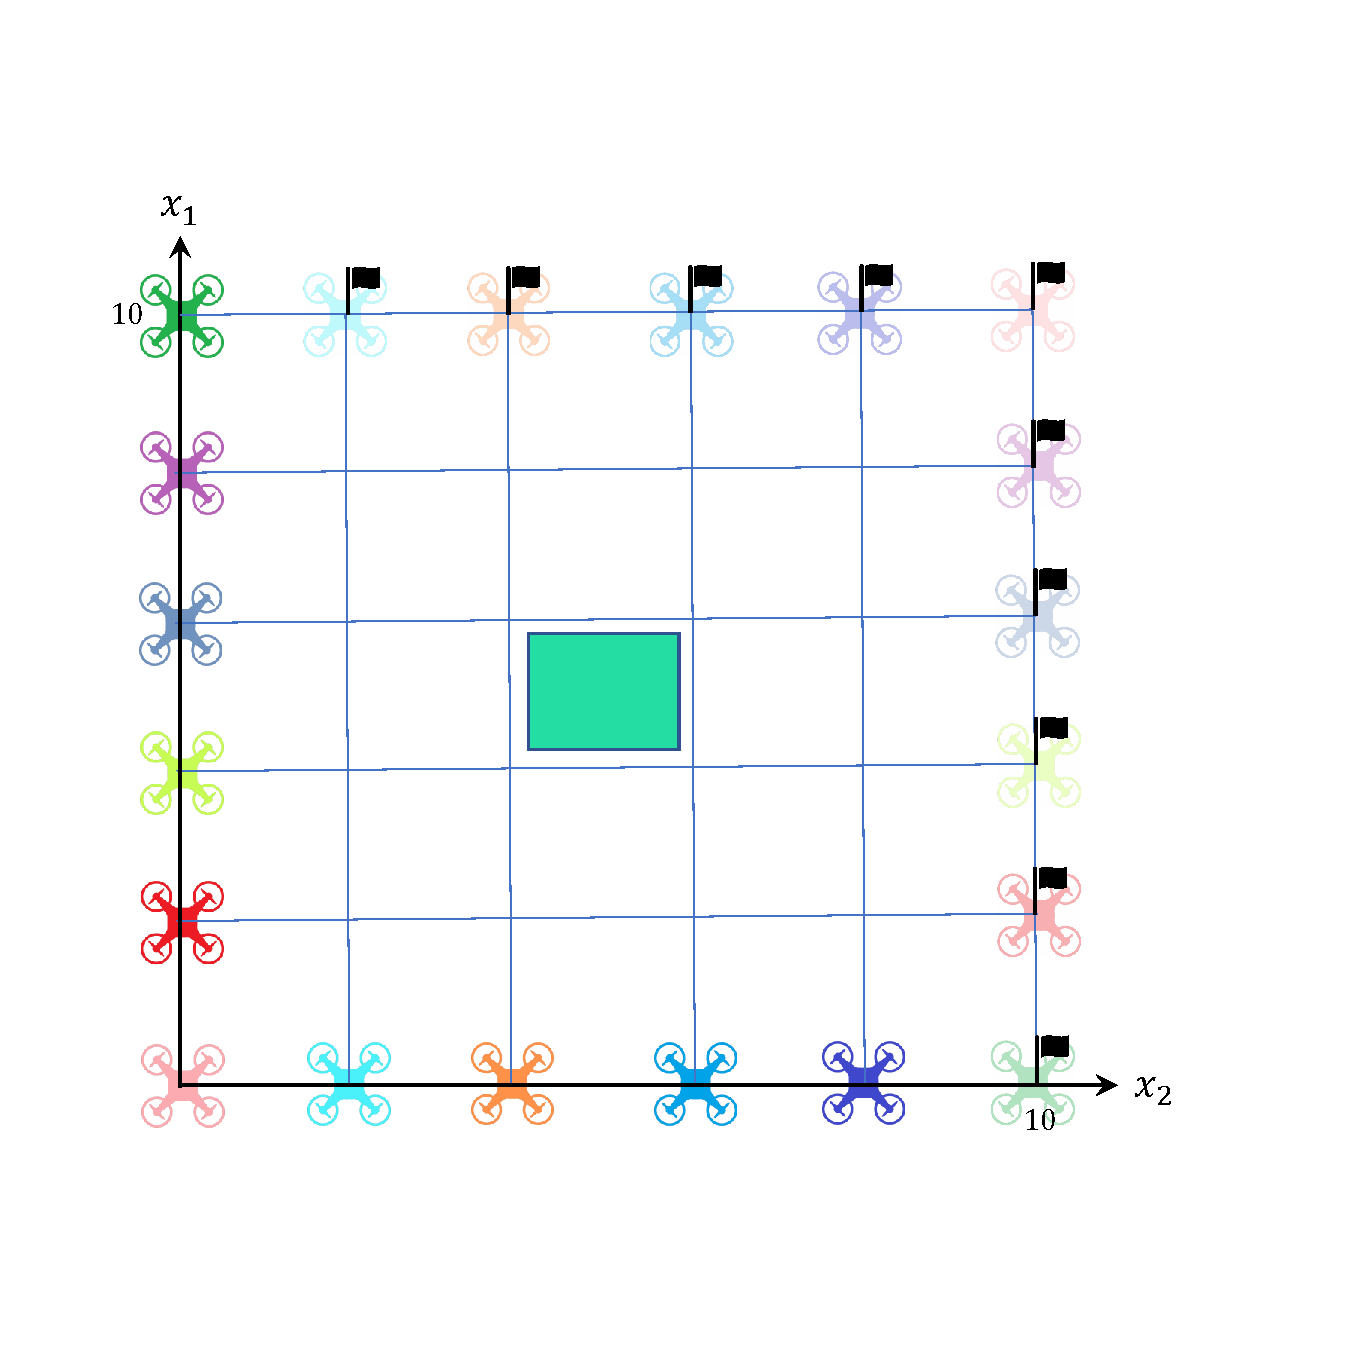
\includegraphics[width=0.45\textwidth]{figures/MA1.pdf}
	\caption{The mission map for the multi-drone path planning example}
	\label{fig:MA}
\end{figure}

\begin{figure}[t]
	\centering
	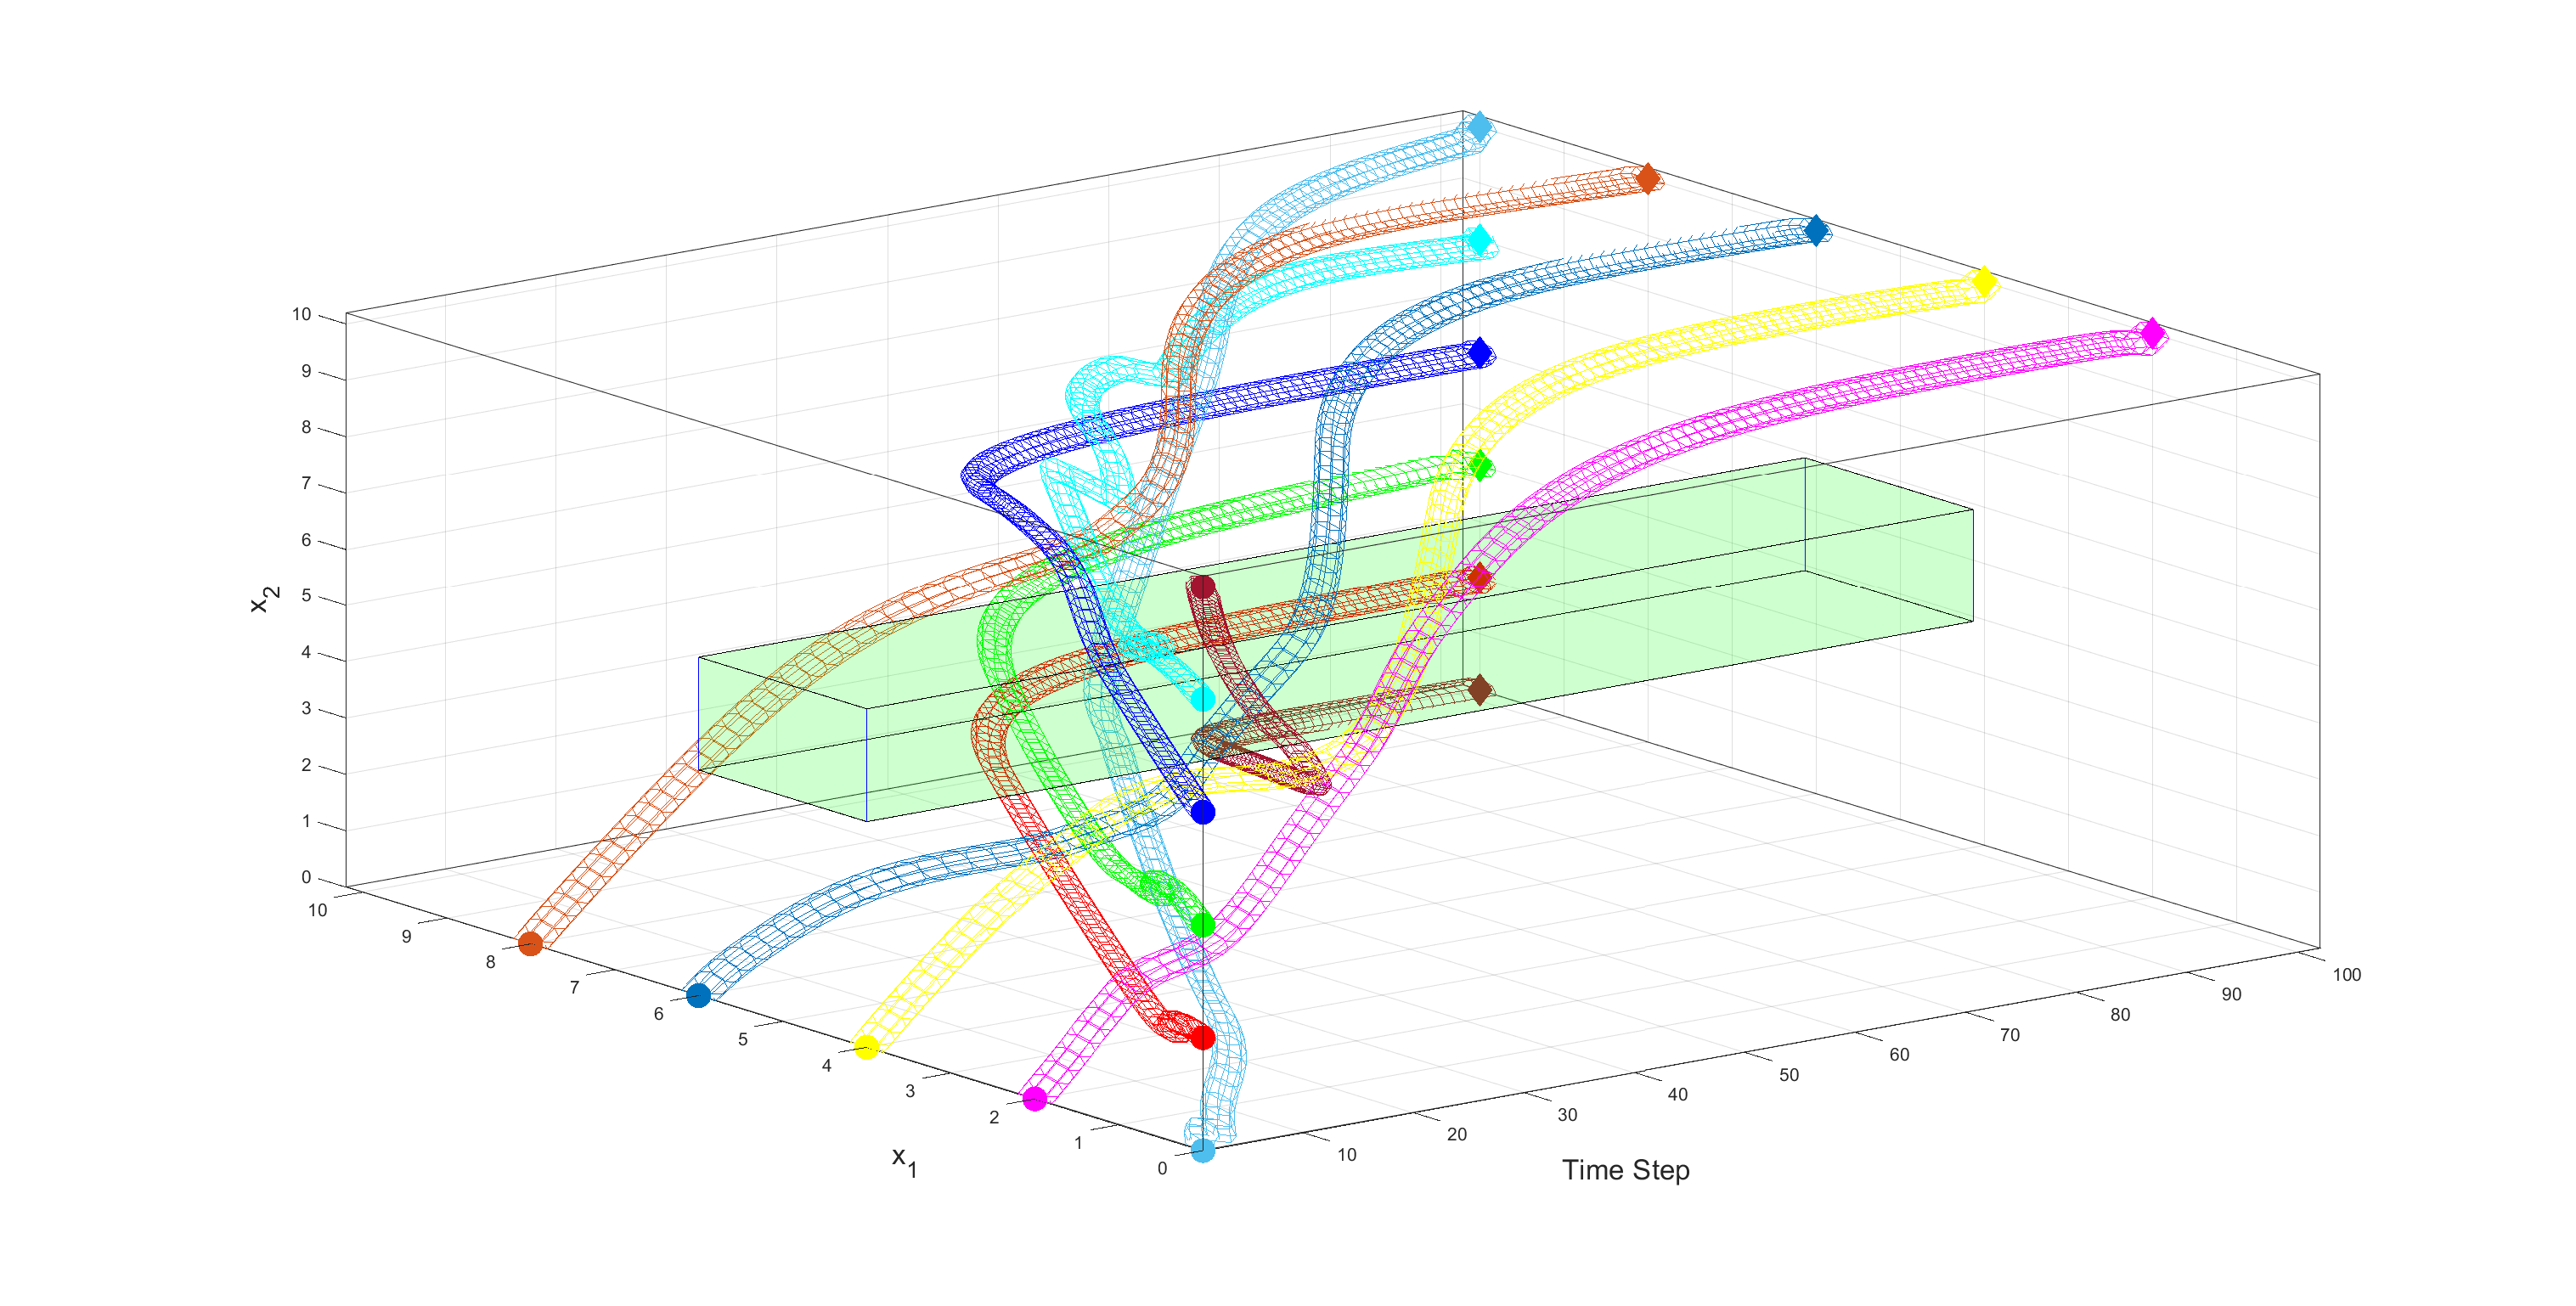
\includegraphics[width=0.45\textwidth]{figures/tubes10.eps}
	\caption{Time-state space illustration of tubes enclosing nominal trajectories for the multi-drone path planning}
	\label{fig:3dtubes}
\end{figure}

\begin{figure}[t]
	\centering
	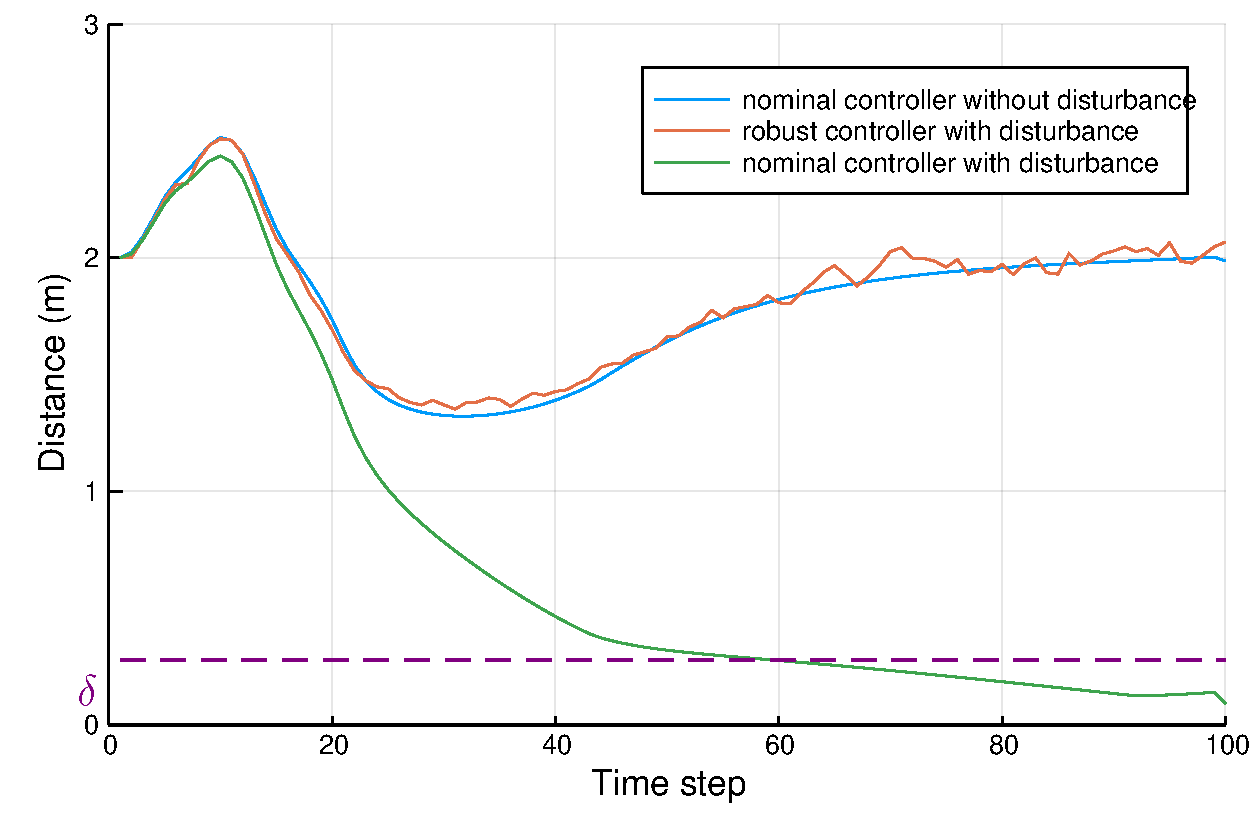
\includegraphics[width=0.45\textwidth]{figures/dist_path_planning.pdf}
	\caption{Performance of open-loop and feedback controllers in regulating distance between drones for disturbance-free and perturbed situations for the multi-drone path planning example}
	\label{fig:multi_drone_distance}
\end{figure}


%In this example, we are focusing on number of robots. This example consist of 10 identical unicycle model. Each unicycle should start from its own initial point and reach target set which is shown in Fig. \ref{fig:MA} with green points and red points. while it avoids obstacles and collision with other agents. Unicycle model is described in below.
%\begin{equation}\label{eq:unicycle_ss}
%	f^{u}(x(t),u(t))=
%	\begin{bmatrix}
%	\dot{x_1}\\
%	\dot{x_2}\\
%	\dot{x_3}
%	\end{bmatrix}=
%	\begin{bmatrix}
%	u_1cos(x_3)\\
%	u_1sin(x_3)\\
%	u_2
%	\end{bmatrix}.
%\end{equation}
%In Eq. \ref{eq:unicycle_ss} $u_1$ is linear speed and $u_2$ is  angular speed and $x_1$ and $x_2$ represents positions and $x_3$ is the angle. Here goal of the problem is designing a controller which satisfy the specifications which mentioned in sec. \ref{sec:Problem_statement}. For this purpose, According to sec.\ref{sec:nominal trajectory} at first we combine all of unicycle dynamics to create a centralized model of the centralized system. The centralized system has $10\times3$ dimension for state space and $10\times2$ dimension for input space. For collision avoidance and obstacle avoidance we use $\delta_{col}=1.5$ and $\delta_{obs}=2$ and we use euclidean distance as a metric for distance in 2D space. In this step, we solved mentioned problem with ALTRO with sample time 0.05 and 200 points for trajectory. Computation takes 138 seconds. Result of ALTRO is illustrated in fig \ref{fig:MA}. 
%In next step we synthesize close loop controller using ABCD with $\varepsilon=[0.16,0.16,0.16]$.  As we mentioned in Prob. \ref{alg:abcd-with-time-for-tracking} we are going to to design a controller that is able to track the trajectory with $\varepsilon$ distance in every time step which is also robust to the disturbance .\MZ{Here we can split the centralized system to 10 separate system and design a close loop controller for each one of them separately.} In order to do this step, we select $\varepsilon$ in a way that it satisfies $\delta_{col} > 2\sqrt{\varepsilon_x^2+\varepsilon_y^2}$ (since tubes should not intersect with each other). Then we are able to design a controller guaranteeing the specifications for each agent independently using Alg. \ref{alg:abcd-with-time-for-tracking} and SCOTS. We select parameters in this way:\\
%$\widetilde{X}=[-1:11]*[-1:11]*[-\pi,\pi]*[0,1]$\\
%$U=[-3,3]*[-3,3]$\\
%$\eta_{\widetilde{X}}=[0.04,0.04,0.04,0.05]$\\
%$\eta_{U}=[0.6,0.6]$\\
%number of states = about $7*10^7$\\
%reduced number of states = about $7*10^7$\\
%number of inputs =121\\
%
%Abstraction in total for 10 systems takes about 12 minutes(average 100 seconds for each system) and synthesizing controller takes about 2 minutes(near 15 seconds for each system). Controller designed in this way is able to overcome bounded additive disturbance $|w|\leq[0.03,0.03,0.03]$ (for all of unicycles). Nominal controller which is produced by ALTRO with presence of this disturbance will be pushed outside of $\epsilon$ tube and also as it shown in the Fig.\ref{fig:MA}, trajectory 1 and 2 will have collision with this value of disturbance. 




 %Figure~\ref{fig:inv_pend} demonstrates variations of disturbance limit under which SCOTS is able to find a controller for different tube width. %It can be observed that by increasing the tube width, SCOTS is able to synthesize a controller for larger disturbance levels. Figure~\ref{fig:invpend_traj} demonstartes trajectories of the system  \eqref{eq:inv_pend_ssq} governed by controllers synthesized by ALTRO and SCOTS under appliance of constant disturbance vector \MS{$[??,??]$}. As expected, the controller designed by ALTRO is not able to tackle disturbance, while using the controller generated by SCOTS, the trajectory remains within the desired bound.

%\begin{figure}\label{fig:inv_pend}
%	\includegraphics[]{}
%	\caption{Variations of disturbance limit for which SCOTS is able to find a controller with tube size}
%\end{figure}
%\begin{figure}\label{fig:invpend_traj}
%	\includegraphics[]{}
%	\caption{}
%\end{figure}
%\textcolor{red}{
\subsubsection{Crane and Vehicle}
\label{subsec}
The goal of this example is to study performance of our method for controlling a number of robots with different dynamics. %Consider a production line wherein a crane (modeled as a cart-pole system) puts some items at certain points and a forklift is in charge of picking these items up. It is assumed that at its lowest height the crane's hook is positioned such that the forklift cannot pass. In particular, Fig.~\ref{fig:cr_and_lft_2} shows a scenario wherein the crane (initially positioned toward left of the boom) needs to unload at the other end of the boom. At the same time, the forklift (initially positioned near the right end of the boom) needs to pick some item locating near the left end of the boom. The goal is to control both the crane and the forklift so that the forklift reaches the object without colliding with the crane. 
We model the crane and vehicle by tuples $\Sigma^1=(X^1,x_\init^1,U^1,W^1,f^c)$ and $\Sigma^2=(X^2,x_\init^2,U^2,W^2,f^l)$, respectively. The crane is modeled as cart-pole system with the dynamical model taken from \cite{Barto1983}:
\begin{align*}
	\ddot{\theta} &= \frac{M_tg\sin(\theta) - \cos(\theta)(F + M_pl \dot{\theta}^2 \sin(\theta))}{l(4/3 M_t- M_p \cos^2(\theta))}=f^c_1(\theta,\dot{\theta},F)\\
	\ddot{z}&= \frac{F + M_pl \dot{\theta}^2 \sin(\theta)-M_pl \ddot{\theta} \cos(\theta)}{M_t}=f^c_2(\theta,\dot{\theta},F),
\end{align*}
where
\begin{itemize}
	\item[] $g=-9.8$ $m/s^2$ is the acceleration of gravity,
	\item[] $M_c=1$ kg is the cart mass,
	\item[] $M_p=0.1$ kg is the pole mass,
	\item[] $M_t=M_c+M_p$ denotes the total mass,
	\item[] $l=0.5$ m is the half-pole length.
\end{itemize}
Further, cart's position, pole's angle and input force to the cart are denoted by $x_1^{(1)}=z$, $x_3^{(1)}=\theta$ and $u^{(1)}=F$, respectively. State space model of the crane is of the following form:
 %for which the set of state variables $X^1$ consists of $x_1^{(1)}$, $x_2^{(1)}$, $x_3^{(1)}$ and $x_4^{(1)}$ denoting (linear) position and speed of the cart and (angular) position and speed of the pole, respectively. The set of input variables includes $u_1^{(1)}$ which represents linear acceleration of the cart. Finally, crane's dynamics takes the form for an inverted pendulum (see, e.g., \cite{barto1983neuronlike}) and can be written as
\[f^{c}(x^{(1)}(t),u^{(1)}(t))=\begin{bmatrix}
	\dot{x}_1^{(1)}\\
	\dot{x}_2^{(1)}\\
	\dot{x}_3^{(1)}\\
	\dot{x}_4^{(1)}
\end{bmatrix}=\begin{bmatrix}
\dot{z}\\
\ddot{z}\\
\dot{\theta}\\
\ddot{\theta}
\end{bmatrix}=
\begin{bmatrix}
	x_2^{(1)}\\
	f^c_1(x_3^{(1)},x_4^{(1)},u^{(1)})\\
	x_4^{(1)}\\
	f^c_2(x_3^{(1)},x_4^{(1)},u^{(1)})\\
\end{bmatrix}.\]
%with
%\begin{align}
%	f^c_2(x{(1)},u^{(1)})=\frac{g\;\sin(x_3^{(1)})}{}
%\end{align}
%\MS{what are $f^c_1$ and $f^c_2$?}
%The output mapping for the crane is defined as
%\[
%h^c(x^{(1)}(t))=\begin{bmatrix}
%	x_1^{(1)}+l \sin(x_3^{(1)})\\
%	y_1+l \cos(x_3^{(1)})
%\end{bmatrix},
%\]
%where, $y_1>0$ is a constant that denotes the cart's height from the ground.
The vehicle's dynamics takes the form
\[f^{l}(x^{(2)}(t),u^{(2)}(t))=\begin{bmatrix}
\dot{x}_1^{(2)}\\ \dot{x}^{(2)}_2 \end{bmatrix}=\begin{bmatrix} x^{(2)}_2\\ u^{(2)} \end{bmatrix},
\]
where $x_1^{(2)}$ and $x_2^{(2)}$ denote the vehicle's position and speed and $u^{(2)}$ represents the vehicle's control input (acceleration). %The output mapping for the crane is defined as
%\[
%h^l=\begin{bmatrix}
%	x_1^{(2)}\\
%	y_2
%\end{bmatrix},
%\]
%where, $y_2>0$ is a constant that denotes the height of the forklift's head with respect to the ground.

%As promised, we use ALTRO in the first step to generate a valid trajectory for the case that $W=\{0\}$. 
There is no obstacle for this example and for minimum distance between the crane and the vehicle we choose $\delta=\begin{bmatrix}0.035&0.2\end{bmatrix}^T$. The sampling time and the horizon length are fixed to $\tau=0.1$ and $T=70$, respectively. Given these settings, ALTRO was capable of generating a valid nominal trajectory in $0.65$ seconds. Fig.~\ref{fig:cr_and_lft_2} (\textbf{left}) demonstrates snapshots of the produced trajectory. Surprisingly enough, applying (constant) additive disturbance $W=\begin{bmatrix}0&0.05&0&0\end{bmatrix}^T$ (to the cart-pole system) causes collision between the crane and vehicle before the end of the mission (Fig.~\ref{fig:cr_and_lft_2} (\textbf{right})).

In the next step, we use SCOTS in order to compute a feedback controller tolerating additive disturbance $|W^1|\leq\begin{bmatrix}0&0.05&0&0\end{bmatrix}^T$ for the crane and $|W^2|\leq\begin{bmatrix}0&0.1\end{bmatrix}^T$ for the vehicle. %We note that the selection of tube sizes need to satisfy the following inequality:
%\[ \delta_{col}> \varepsilon_{1}^{(1)} + l\times\varepsilon_{3}^{(1)} + \varepsilon_{1}^{(2)},\]
%where $\varepsilon_{1}^{(1)}$, $\varepsilon_{3}^{(1)}$ denote tube sizes over $x_1^{(1)}$ and $x_3^{(1)}$, $l$ denotes the length of the rope between the cart and the hook and $\varepsilon_{1}^{(2)}$ denotes the tube size over $x_1^{(2)}$. 
We choose state and input spaces for the crane to be $X^{1}=[-0.195,5.49]\times[-1.99,4.37]\times[1.20,4.68]\times[-5.44,5.28]$ and $U^{1}=[-7,7]$, respectively. For the vehicle, we set $X^{2}=[3,9]\times[-3,1.995]$ and $U^{2}=[-3,3]$. %Next, we augment both dynamics with time and 
Next, we choose state and input partition sizes $\eta_{{X}}^{1}=\begin{bmatrix}0.015&0.035&0.016&0.064\end{bmatrix}^T$, $\eta_{U}^1=0.2$,  $\eta_{{X}}^2=\begin{bmatrix}0.01&0.015\end{bmatrix}^T$ and $\eta_{U}^2=0.1$. These selections yield discretized models with state and input spaces having $2.5\times 10^9$ and $71$ points for the crane, and $2\times 10^5$ and $61$ points for the vehicle. Next, we limit both of the state spaces into tubes constructed around the open-loop trajectories with sizes specified as $\varepsilon^{1}=\begin{bmatrix}0.135&0.385&0.176 &0.768\end{bmatrix}^T$ and $\varepsilon^{2}=\begin{bmatrix}0.08&0.12\end{bmatrix}$. This reduces size of state spaces into $1.2\times 10^7$ and $1.5\times 10^4$ for the crane and vehicle, respectively. Given the above settings, SCOTS was able to compute abstraction in $511$ and $0.22$ seconds for the crane and the vehicle, respectively. Scots performs synthesis in $91$ and $0.037$ seconds for the crane and the vehicle, respectively.
			
%\begin{figure}[t]
%	\centering
%	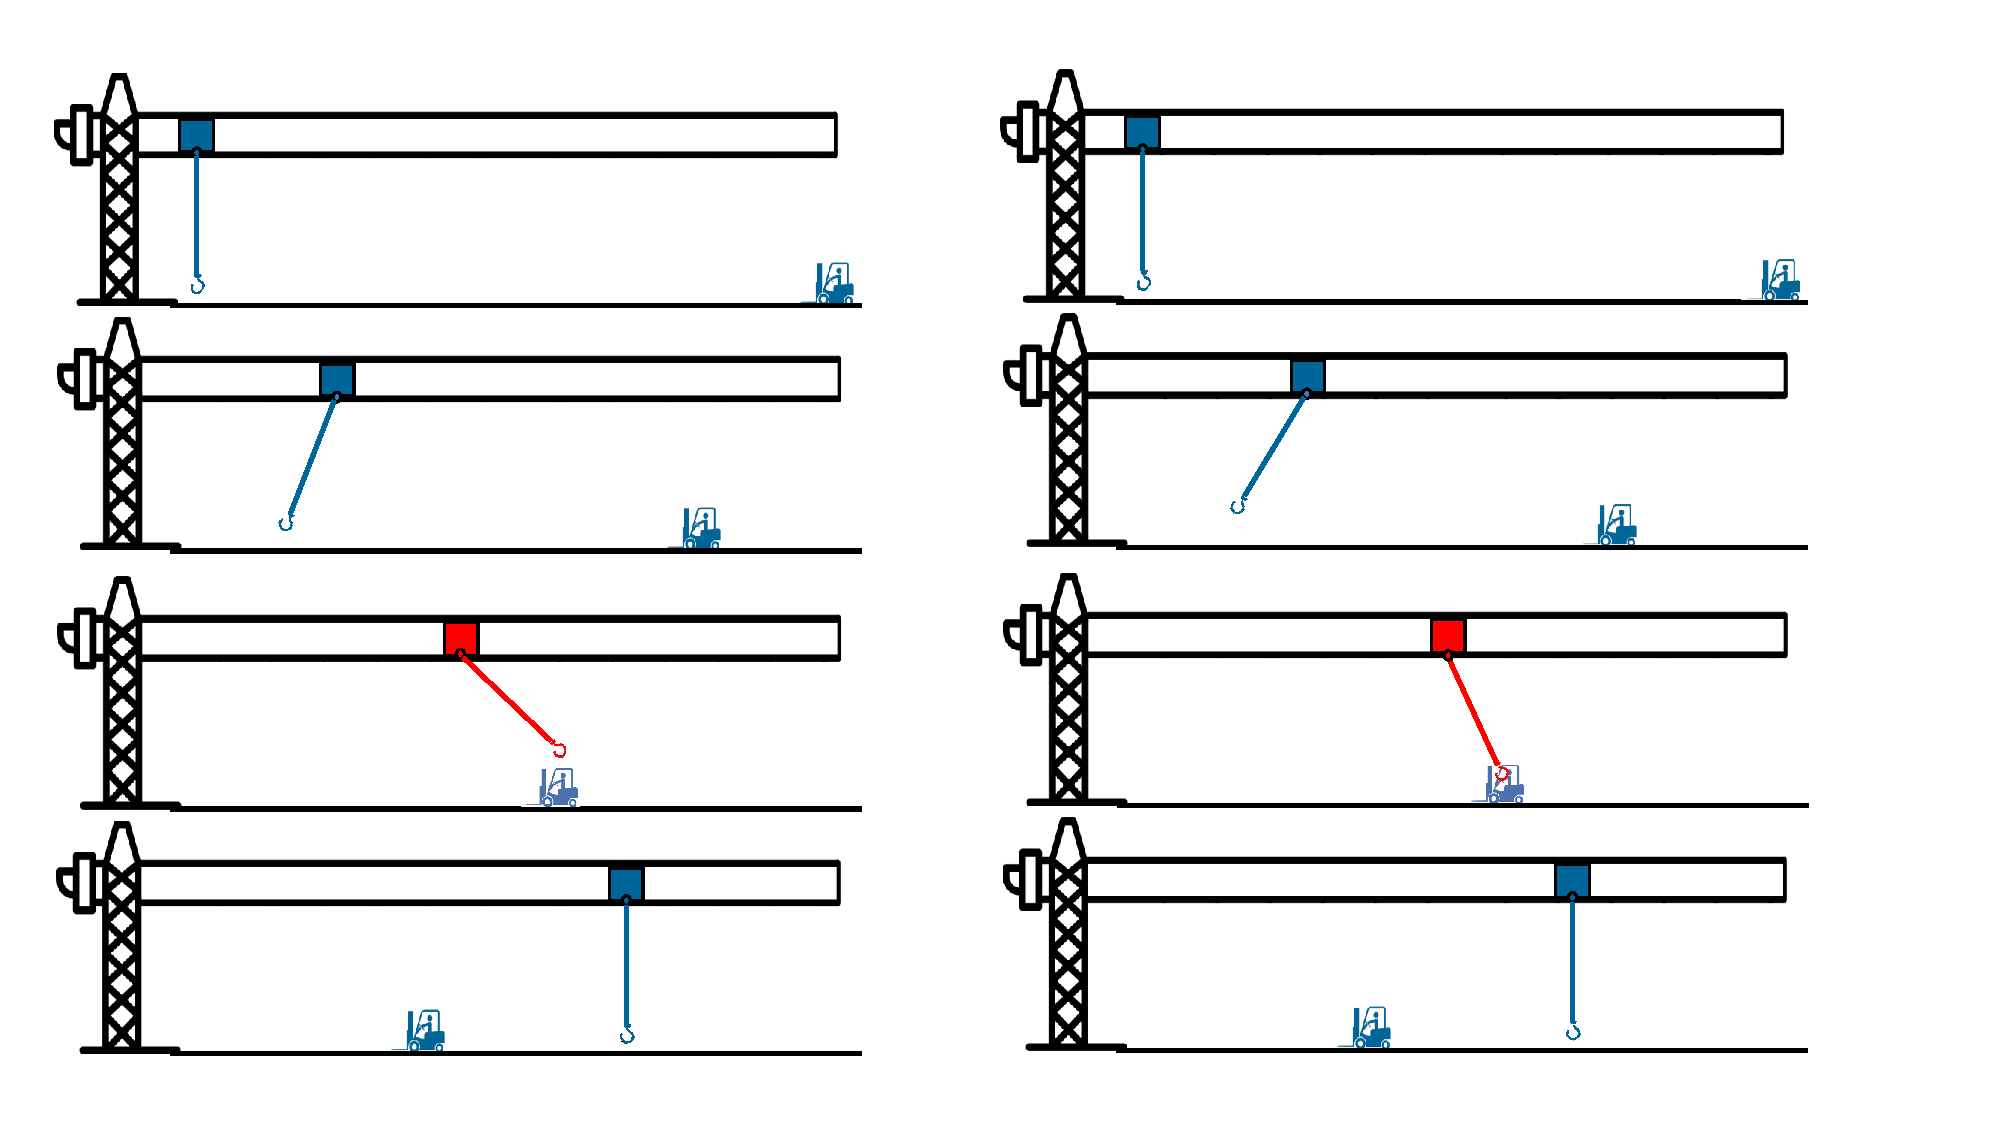
\includegraphics[width=0.45\textwidth]{figures/crane_and_forklifter.pdf}
%	\caption{Illustration of the trajectories generated by the open-loop controller for the crane and vehicle example under disturbance-free (\textbf{left}) and perturbed (\textbf{right}) situations} 
%	\label{fig:cr_and_lft_2}
%\end{figure}


%In this example, we show the method can handle multiple heterogeneous dynamical systems. This example is Modelling a special situation in a factory(shown in fig \ref{fig:cr_and_lft}) . Assume there is a crane and and a forklift. Each one of them should reach their destination without having any accident(satisfying specs). The Crane position will change from 0 to 5 and the forklift from 9 to 4.  Here we model the forklift using $\begin{bmatrix} \dot{x_1}\\ \dot{x_2} \end{bmatrix}=\begin{bmatrix} x_2\\ u \end{bmatrix}$ ($x_1$ and $x_2$ are representing position and velocity) and for the crane we use inverted pendulum model with exactly same configuration in \cite{barto1983neuronlike}: \\ 
%\[\begin{bmatrix}
%\dot{x}\\
%\Ddot{x}\\
%\dot{\theta}\\
%\Ddot{\theta}
%\end{bmatrix}=\begin{bmatrix}
%\dot{x_1}\\
%\dot{x_2}\\
%\dot{x_3}\\
%\dot{x_4}
%\end{bmatrix}=\begin{bmatrix}
%x_2\\
%g(x_3,x_4,u)\\
%x_4\\
%f(x_3,x_4,u)\\
%\end{bmatrix}\]
%
%where $x$ represent position of the cart  and $\theta$ is angle of the pole, f and g are non-linear functions. The process of controller design is similar to Sec. \ref{sec:MultiAgent}; At first we find a nominal trajectory with ALTRO with required specifications then we robustifing it using our method with modified ABCD.\\
%In this example we do not have any static obstacle, but for collision avoidance we use euclidean distance as the metric with $\delta=0.4$ for measuring distance between crane and forklift. We consider hook of crane as a point mass with a radius and forklift as several point mass on circumference of it, So we consider minimum distance between the hook and points of the forklift as the distance. ALTRO solve this trajectory generation problem using sampling time =0.1 and number of points=40 in 10.7 seconds.\\
%to guarantee collision avoidance specification we should select tube sizes to satisfy:
%\[ \delta_{col}> \varepsilon_x + l*\varepsilon_\theta + \varepsilon^\prime_x\]
%where $\varepsilon_x$ and $\varepsilon_\theta$ are tube sizes for position and angle in crane model (cart pole) and l is the length of the joint and $\varepsilon^\prime_x$ is tube size for position of the forklift.
%In next phase we use finite abstraction with $\varepsilon_x=9*0.015$ and $\varepsilon_\theta=11*0.015$ and $\varepsilon^\prime_x=9*0.015$. It takes about 1000 seconds for crane (cart-pole system) with (1.15)*($10^{11}$) number of input-states pairs and ($7*10^6$)*(71) reduced number of states and synthesis takes 35 seconds. For forklift abstractions abstraction and synthesis will finish in less than a second.\\
%The nominal controller with disturbances $w_1=[0,0.02,0,0]$ for crane and $w_2=[0,0.1]$ for forklift will fail collision specification.
%
%


%} 


\subsubsection{Lane Merging}
Finally, we study a lane merging problem wherein multiple controlled vehicles are driving over two merging lanes (Fig.~\ref{fig:merge}, \textbf{top} frame). A dangerous situation may occur at the merging point of the two lanes if vehicles are not controlled properly. Different variants of this problem has been studied in the literature (see, e.g., \cite{xiao2019merging,xiao2020merging}). Without seeking to optimize fuel consumption or travel time, we set the goal to control the vehicles to pass the merging zone safely. In particular, consider a situation where initially three cars are driving on each of the two lanes (Fig.~\ref{fig:merge}, (\textbf{top})). The control objective for each vehicle is to pass the red dashed line within a finite horizon without hitting the road's sides or colliding with other vehicles. 

%Every vehicle is modeled as tuple $\Sigma=(X,U,W,f^v,Y,h^v)$. 
%Dynamics for each vehicle takes the form
%\begin{equation*}\label{eq:vehicle_ss}
%	f^{v}(x(t),u(t))=
%	\begin{bmatrix}
%		\dot{x_1}\\
%		\dot{x_2}
%	\end{bmatrix}=
%	\begin{bmatrix}
%		u_1\\
%		u_2
%	\end{bmatrix},
%\end{equation*}
%where $x_1$, $x_2$ denote the vehicle's position in $2D$ plane, $u_1$ and $u_2$ represent the vehicle's speed coordinates, respectively. The output mapping is defined as
%\[
%h^v(x(t))=x(t).
%\]
The model for each of the vehicles is the same as the drone model given in Sec.~\ref{sec:Multirobot} ($\Sigma^i=(X,x_\init^i,U,W,f^d)$). For collision and obstacle avoidance, we choose $\delta=\begin{bmatrix}0.37&0.37\end{bmatrix}^T$. The sampling time and the horizon length are fixed to $\tau=0.1$ and $T=110$, respectively. Given these settings, ALTRO generates a valid nominal trajectory in $100$ seconds. Next, we use SCOTS in order to compute a feedback controller tolerating additive disturbance $|W|\leq\begin{bmatrix}0.03&0.03&0.03\end{bmatrix}^T$. We choose state and input spaces for each vehicle's model to be $X=[-0.5,15]\times[0.1,7.4]\times[-1,0.4]$ and $U=[-0.9,3]\times[-2.1,2.1]$, respectively. State and input partition sizes are chosen as $\eta_{X}=\begin{bmatrix}0.02&0.02&0.02\end{bmatrix}^T$ and $\eta_{U}=\begin{bmatrix}0.3&0.15\end{bmatrix}^T$. These selections yield discretized models with abstract state and input spaces having $2.1\times 10^7$ and $406$ points. Next, we limit the state spaces into tubes constructed around the open-loop trajectories with sizes specified as $\varepsilon=\begin{bmatrix}0.16&0.16&0.16\end{bmatrix}^T$. This reduces size of state space into $1.9\times 10^5$ (in average). Given the above settings, SCOTS was able to compute abstraction in $159.6$ seconds ($26.6$ seconds in average) and synthesize controllers in $40.8$ seconds ($6.8$ seconds in average). Fig.~\ref{fig:merge} demonstrates snapshots of one sample trajectory when feedback controllers are employed under the presence of disturbance. Fig.~\ref{fig:multi_drone_distance} illustrates the fact that open-loop controller fails in keeping one of the vehicles away from the road's sides under perturbed situation when constant additive disturbance vector $\begin{bmatrix}-0.03 &0.03&-0.03\end{bmatrix}^T$ is being applied throughout the whole horizon. In contrast, emplying feedback controller results in successful lane merging. %Fig.~\ref{fig:multi_drone_distance} illustrates performance of open-loop and feedback controllers on regulating distance between of the vehicles from the road's sides with and without disturbance. In the absence of disturbance open-loop controller is capable of maintaing a minimum distance from the road's sides. Next, we consider the case when constant additive disturbance vector $\begin{bmatrix}-0.03 &0.03&-0.03\end{bmatrix}^T$ is being applied to the vehicle throughout the whole horizon. It can be noticed that applying the open-loop controller causes that distance from the road's side (shown in solid red) becomes smaller than $\delta$. However, the feedback controller is still capable of maintaining distance above the given threshold (shown in solid green).





%
%consider the situation which is found in ref[??]. In this situation we consider 6 numbers of car in two different lanes(merging lane and main lane) . Here the goal is reaching the red line ( x position should get bigger than 15) which is shown in fig ?? while they satisfying specifications ( avoid collision with other cars and border of lanes) .
%Number of cars is fixed it means number of cars not changing during simulation time. but it also doesn't mean all of the cars reach the target at same time.\\
%The problem that we are solving has several differences with the example on the paper. they optimize time and fuel for each car and tehy consider several constraints for speed and positions. they also consider 2d linear model for each car. Here we only try to solve the reachability problem. we consider reach top speed limitation and angle acceleration and lanesborders As constraints. For each car we consider the model represented in eq[6] (same model as multi-car example) which has more dimension and is nonlinear.



\begin{figure}
	\centering
	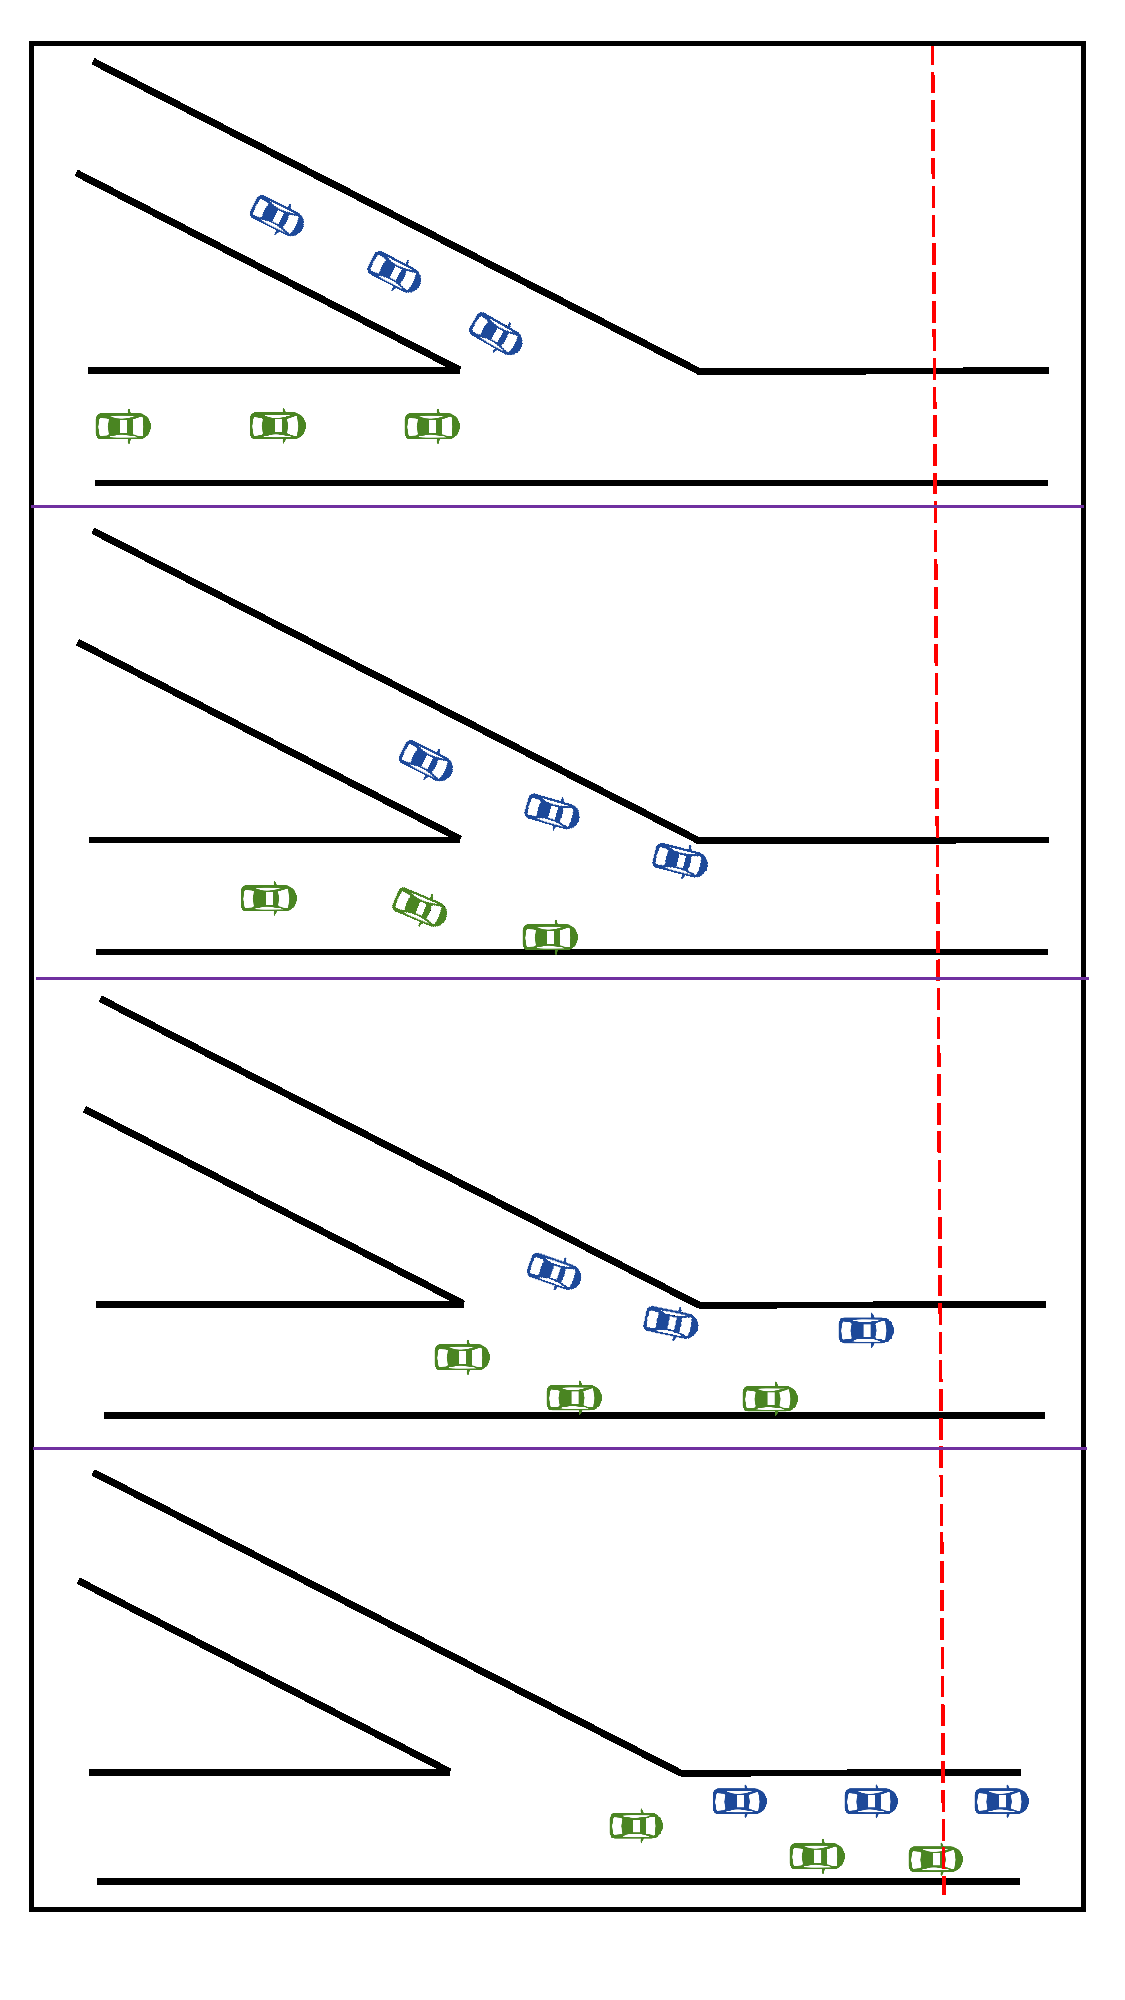
\includegraphics[width=0.45\textwidth,height=0.4\textheight]{figures/merge.pdf}
	\caption{Illustration of a (sample) trajectory generated by formally guaranteed feedback controllers for the lane merging example}
	\label{fig:merge}
\end{figure}

\begin{figure}[t]
	\centering
	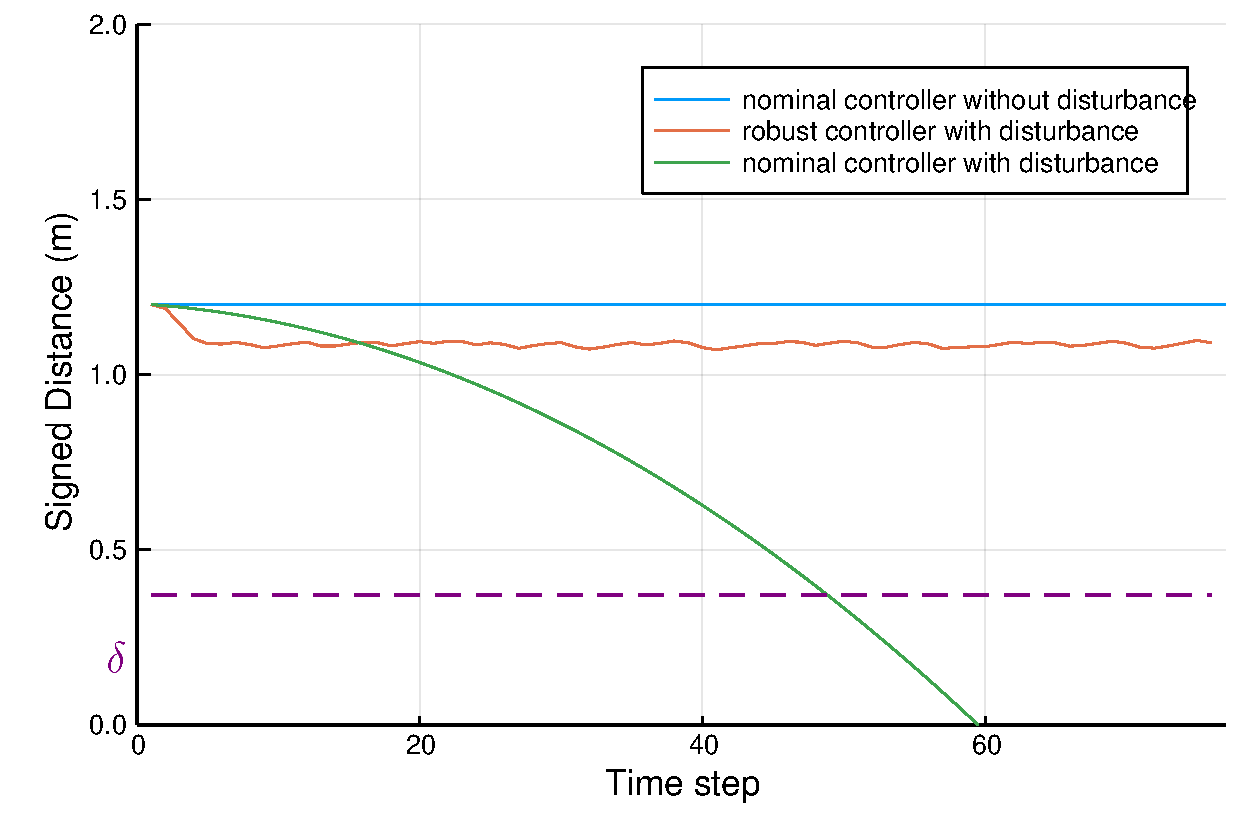
\includegraphics[width=0.45\textwidth]{figures/dist_merging.pdf}
	\caption{Performance of open-loop and feedback controllers in regulating distance between drones for disturbance-free and perturbed situations for the lane merging example}
	\label{fig:merging_distance}
\end{figure}


\subsection{Global formation control problem}\label{sec:global formation control}

The second category of example, that we are about to present, is about maintaining a global formation while satisfying a set of reach-avoid specifications.
We show how the formation control problem can be expressed using a static obstacle $\avoid$ on the product state space $X^\times$, as required by the problem setup in Sec.~\ref{sec:problem}.

Let us first formalize the notion of formation.
Let $\Set{\Sigma^i=(X^i,x_\init^i,U^i,W^i,f^i)}$ be a set of robots.
A \emph{formation constraint} is a set $\Set{\lambda^{i,j}\in \mathbb{R}}_{i,j\in [1;N]}$ where every $\lambda^{i,j}$ specifies the relative \emph{euclidean} distance between the projections of state of robot $\Sigma^i$ and robot $\Sigma^j$ over the shared output space $Y$.
(We use euclidean distance to define formation, as opposed to the distance $D$ used in the rest of the paper, to allow rotation of the formation while moving.)

Now suppose $\goal^i\subseteq X^i$ is the individual goal states, $\obs\subseteq Y$ is a common obstacle in the output space, $\delta \in \mathbb{R}^p_{>0}$ is a safety margin, and $\mu\in \mathbb{R}^p_{>0}$ is a tolerance margin for the formation constraint.
The formation control problem then asks to generate controllers $\set{C_i}$ such that every robot $\Sigma^i$ eventually reaches $\goal^i$ while avoiding $\obs$ by the margin $\delta$, as well as while making sure that the \emph{euclidean} distance between robot $\Sigma^i$ and $\Sigma^j$ is in the range $\lambda^{i,j} \pm \mu$.
Essentially the tolerance margin $\mu$ is to account for the possible slight deviations due to disturbances experienced by the robots. Notice that since the robots have their own goals, and at the same time they need to ``stay close'' to their neighboring robots in the formation for the entire period, hence they might first need to accompany the other robots to their goals, before being accompanied by them to reach its own goal.

Let $D_e\colon \mathbb{R}^n\times \mathbb{R}^n\to \mathbb{R}^p_{\geq0}$ denote the euclidean distance.

We can express the formation control problem in the product state space as follows:
\begin{itemize}
	\item The goal set $\goal\subseteq X^\times$ is defined as $\goal \coloneqq \goal^1\times \ldots \times \goal^N \subseteq X^\times$, and
	\item The static obstacle $\avoid\subseteq X^\times$ is defined as 
		\begin{align}
			&\avoid \coloneqq\nonumber\\ 
			&\Set{ x\in X^\times | 
				\begin{array}{c}
					\exists i\in [1;N]\;.\; D(\proj^i(x),\obs) \leq \delta\\
					\vee\\
					\exists (i,j)\in [1;N]\times [1;N]\;.\;\\ D_e\left(\proj^i(x),\proj^j(x)\right)\notin\lambda^{i,j}\pm \mu
			\end{array}},					
		\end{align}
\end{itemize}
where the last disjunction in the definition of $\avoid$ is the restriction required for maintaining the formation, and the rest are same as in Sec.~\ref{sec:local reach-avoid}.
Once the sets $\goal$ and $\avoid$ are obtained as above, we can use Alg.~\ref{alg:main} to find the set of feedback controllers $\set{C^i}$.

%\todo{The example goes here...}
\subsubsection{Multi-drone formation control}
\label{subsec:formation_control}
Consider a formation control scenario where a set of five drones (identically modelled) need to go from a specified start point to a certain destination (both defined over the corresponding state spaces) within a finite horizon, while four of them forming a diamond around a fifth drone (positioned at the diamond's center) at every time point. There are two square-shaped obstacles (defined over the output space) from which the group needs to keep a certain minimum distance at all of the time points. %As mentioned before, to check the formation the relative positions between the $i^{th}$ and $j^{th}$ drones is measured by euclidean norm ($d_e^p(.,.)$) whereas collision/obstacle avoidance is checked by the infinity norm$d^p(.,.)$.

The model for each of the drones is the same as the drone model given in Sec.~\ref{sec:Multirobot} ($\Sigma^i=(X,x_\init^i,U,W,f^d)$). Distance between each pair of drones positioned at the diamond's vertices is set to be $\lambda^{i,j}=\frac{3\sqrt{2}}{2}$ for $i,j\in\set{1,2,3,4}$, while the drone positioned at the center is supposed to keep distance $\lambda^{5,j}=1.5$ for $j\in\set{1,2,3,4}$. Setting the minimum distance for obstacle avoidance to $\delta=\begin{bmatrix}0.4&0.4\end{bmatrix}^T$, sampling time $\tau=0.1$ and horizon length $T=100$, ALTRO finds a valid solution over the product system with $15$ state and $10$ input variables within $163$ seconds.
%Synthesizing local controllers for every drone such that the specifications hold for the perturbed models, is performed similar to the previous examples. 
We follow the steps outlined in Alg.~\ref{alg:abcd-with-time-for-tracking} to synthesize local controllers for every drone such that the specifications hold for the perturbed models with $|W|\leq \begin{bmatrix}0.03&0.03&0.03\end{bmatrix}^T$ and $\mu=0.5$. %We construct a tube around the (nominal) trajectory produced by ALTRO with the width vector $\varepsilon=\begin{bmatrix}??&??&??\end{bmatrix}^T$.
We consider state and input spaces to be $X=[-2,17]\times[-2,17]\times[0.6,1.6]$ and
$U=[-0.9,4.8]\times[-3,3]$, respectively. Choosing state and input partition sizes $\eta_{X}=\begin{bmatrix}0.02&0.02&0.02\end{bmatrix}^T$ and
$\eta_{U}=\begin{bmatrix}0.3&0.15\end{bmatrix}^T$ results in state and input spaces with $10^9$ and $820$ points. 
Computing the transition system over inter-tube space with width $\varepsilon=\begin{bmatrix}0.18&0.18&0.18\end{bmatrix}^T$ results in smaller transition system with $4.9\times 10^5$ points. Given the above settings, SCOTS computes abstraction in $271$ seconds ($54.2$ seconds in average) and $66.5$ seconds ($13.3$ seconds in average). Fig.~\ref{fig:formation_ex} illustrates four sequential frames of a sample trajectory generated by employing feedback controllers. Noticeably, both of the relative position and orientation between drones are kept (almost) constant throughout the journey. Fig.~\ref{fig:formation_distance} illustrates performance of open-loop and feedback controllers on regulating distance between two of the drones with and without disturbance. As expected, in the absence of disturbance open-loop controller suffices and distance between the two drones (shown in solid blue) does not go below the threshold line. However, when constant additive disturbance vectors $\begin{bmatrix}0 &0.03&0.03\end{bmatrix}^T$ and $\begin{bmatrix}0 &-0.03&-0.03\end{bmatrix}^T$ are being applied to the two drones throughout the whole horizon, open-loop controller fails, % that distance between the two drones (shown in solid green) becomes smaller than $\delta$. However, 
whereas the feedback controller is still capable of maintaining distance above the given threshold.

 \begin{figure}[t]
	\centering
	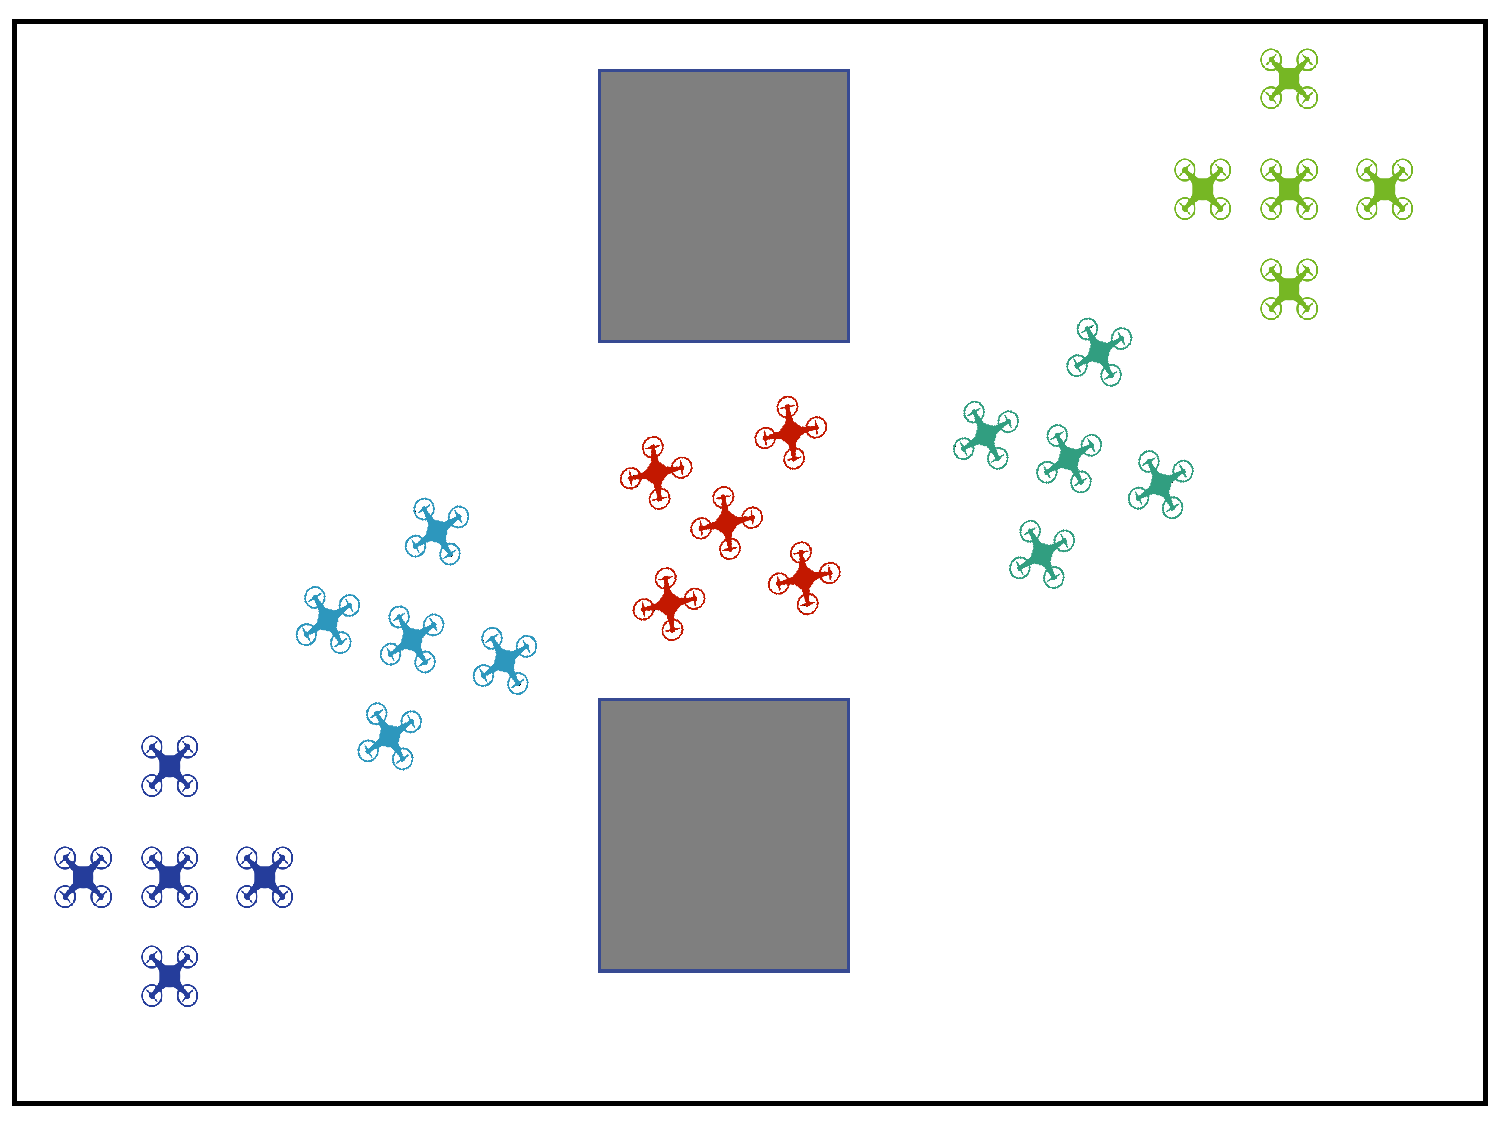
\includegraphics[width=0.45\textwidth]{figures/formation.pdf}
	\caption{Illustration of a (sample) trajectory generated by formally guaranteed feedback controllers for the robot formation control example}
	\label{fig:formation_ex}
\end{figure}

\begin{figure}[t]
	\centering
	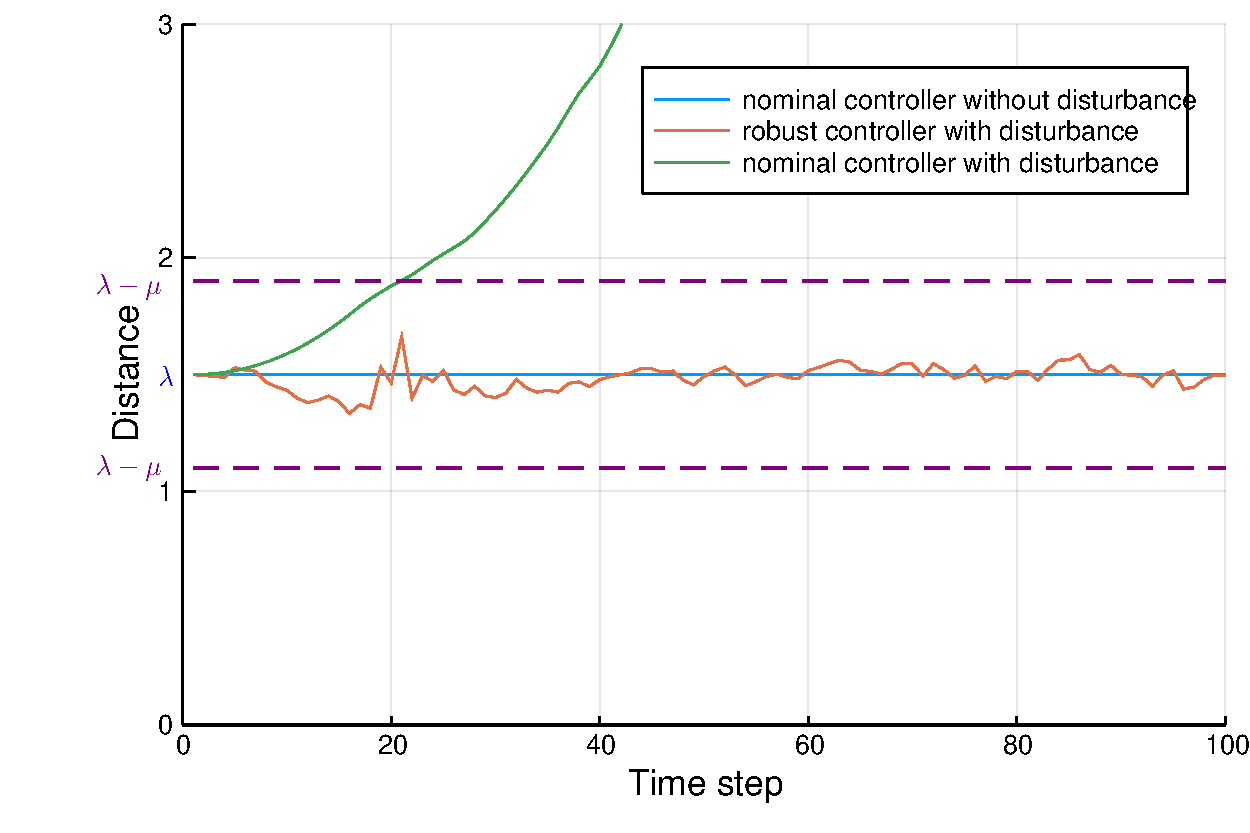
\includegraphics[width=0.45\textwidth]{figures/dist_formation.pdf}
	\caption{Performance of open-loop and feedback controllers in regulating distance between drones for disturbance-free and perturbed situations for the formation control example}
	\label{fig:formation_distance}
\end{figure}
 

%Note that $\delta_{col} > \varepsilon$.
%We use SCOTS in order to synthesize (local) feedback controllers that guarantee reachability, formation control and obstacle/collision avoidance in the presence of bounded disturbance such that $|W|\leq \begin{bmatrix}??&??&??\end{bmatrix}^T$. 
%We consider state and input spaces to be $X=[??:??]^2\times[??,??]$ and
%$U=[??,??]^2$, respectively. Choosing state and input partition sizes $\eta_{X}=[??,??,??]^T$ and
%$\eta_{U}=[??,??]^T$ results in $\hat X$ and $\hat U$ with $??\times ??$ and $??$ points. As we explained in Sec.~\ref{sec:tracking}, we compute the transition system over inter-tube space which has $|\hat P|=??\times ??$ points in this example.%The bound over additive disturbance is set to be $\begin{bmatrix}0.03&0.03&0.03&0\end{bmatrix}^T$. 
%Given the above settings, SCOTS computes abstraction in $??$ minutes for all the drones and synthesizes controllers in about $??$ minutes (in average, abstraction takes $??$ seconds and synthesis takes $??$ seconds). 
%\section{Present Challenges}
%
%\begin{enumerate}
%	\item In some examples, it was necessary to consider a larger control input space for the SCOTS part, than what was used in the ALTRO part.
%	Otherwise, the SCOTS would not be able to track the nominal trajectory within the given precision using any level of discretization. 
%	\item For the ship example, applying the largest disturbance with which SCOTS is able to compute a controller, the trajectory resulted from using the open loop controller does not leave  $\varepsilon-$tube around it; in general magnitude of disturbance for which SCOTS can find a controller is relatively small for most of examples that we have tried.
%\end{enumerate}







\section{Discussion and Future Work}
We have presented a method for synthesizing provably correct decentralized controllers for multi-agent systems with global reach-avoid specifications. 
Our approach is hierarchical: At the top level, we obtain a high-level joint plan by solving a centralized synthesis problem on a simplified model of the product system, and at the bottom level we synthesize local controllers for robustly tracking the high-level plan for each individual agent.
In this section, we discuss different features of our work, remaining challenges, and the future work.

\smallskip
\noindent\textbf{Scalability of the proposed method.}\
We compute the reference trajectory for the product system using ALTRO. Our experiments show that ALTRO generates reference trajectories for high-dimension systems quite fast. On the other hand, for tracking controllers, our method synthesizes controllers in a decentralized manner and thus scalability is not affected by increasing the number of agents. We use SCOTS for computing tracking controllers because the algorithm can be effectively parallelized \cite{KhaledZ19pfaces}. While \tool uses ALTRO and SCOTS for solving the given reach-avoid problem, we emphasize that one could replace them with any other off-the-shelf method that can perform similar tasks.

\smallskip
\noindent\textbf{Comparison to other tools that are able to solve reach-avoid specifications.}\
Our experiments show that our method is efficient in solving reach-avoid tasks for multi-agent systems. However, there are other tools which claim they can solve similar tasks. Table~\ref{tab:tools} lists main features for some of such active tools.
\begin{table*}[t]
	\large
	\centering
	\caption{Features of different tools.}\label{tab:tools}
	\renewcommand{\arraystretch}{1.2}
	\setlength{\tabcolsep}{0.7em} % for the horizontal padding
	%\resizebox{1\columnwidth}{!}{
	\begin{tabular}{l|c|c|c|c|c}
		\toprule
		Tool&Method&
		Dynamics&Type of disturbance&Multi-agent& Method \\
		\midrule
		Ours &Hybrid&non-linear&bounded additive& yes& ALTRO + ABCD \\
		\midrule
		FastTrack\cite{herbert2017fastrack}&centralized&non-linear& bounded(general) & - & RRT + HJ\\
		\midrule
		RealSyn\cite{fan2018controller}&centralized&linear&bounded additive & - & Synthesis\\
		\midrule
		Factest\cite{fan2020fast}&centralized&non-linear & implicit* & - &MILP + lyapanov\\
		\midrule
		Model mismatch(SOS)\cite{singh2018robust} & centralized &non-linear& implicit*  & - &  SOS\\
		\midrule
		RTD\cite{kousik2020bridging}& Centralized &non linear& * & - & NMPC\\
		\midrule
		fly by logic\cite{Pant2018multiquad} & centralized & non-linear & implicit* & yes & optimization\\
		\midrule
		Distributed Trajectory Optimization \cite{jackson2020scalable}&centralized & nonlinear & - & yes & ALTRO\\
		\bottomrule
	\end{tabular}
\end{table*}

\smallskip
\noindent\textbf{Extension to richer classes of specifications.}\
Our proposed method is specific to reach-avoid specifications. However, application of our method can be extended to the problem that can be broken into a sequence of reach-avoid tasks. To that end, one can use high-level languages (e.g., \cite{Majumdar2020,Ghosh2020}) for specifying complex reach-avoid sequences and invoke \tool to solve each individual reach-avoid task.

\smallskip
\noindent\textbf{Choice of parameters.}\
Our algorithm takes as input the robustness margin $\varepsilon$ and the abstraction parameters $\eta_x$ and $\eta_u$.
(The safety margin $\delta$ is also a parameter, but that is considered to be a part of the control problem.)
The larger the value of $\varepsilon$, more difficult it is to synthesize a nominal controller for the product system using ALTRO.
On the other hand, the smaller the value of $\varepsilon$, the more difficult it is to synthesize a set of decentralized controllers using SCOTS.
Also, there is a trade-off between computation time and ease of synthesis when it comes to choosing the parameters $\eta_x$ and $\eta_u$ for SCOTS: Larger values of these parameters will result in faster computation but harder synthesis problem.
Thus there needs to be a good balance when we choose the parameters for our tool.
Indeed, it is not always easy to come up with a good set of parameters.
Our current approach is to add an outer loop around our tool to search of suitable parameters until the decentralized synthesis is successful (see Fig.~\ref{fig:overall}).
In future, we plan to investigate if the parameters can be systematically discovered by separately analyzing the dynamics of the systems.

%\smallskip
%\noindent\textbf{Conservativeness of our method.}\
%Our method is no more conservative than the standard ABCD approach used in SCOTS:
%Indeed, assuming availability of unbounded resources, if SCOTS is able to find a central controller for the global synthesis problem for a given set of parameters $\varepsilon$, $\eta_x$, and $\eta_u$, then our method will also find a set of decentralized controllers (by consuming much less resource than the global synthesis approach).
%\KM{@Mehrdad: is this true? Is it not the case that ALTRO can occassionally fail to give a nominal controller even if the central SCOTS-based approach would have solution, if we would ignore the memory and time limitations?}


%\section{conclusion}
%\MS{We have presented a decentralized controller synthesis scheme for multi-agent systems with global reach-avoid specifications. Our experiments demonstrate effectiveness of our approach for solving reach-avoid problems that may require formation to be preserved. Note that one can connect our work to the high-level languages for robotic applications by formulating more complicated tasks as a sequence of reach-avoid problems together with correct synchronization skleton. It remains to choose the right values of parameters for robustness parameter $\varepsilon$ and discretization parameters $\eta_x$ and $\eta_u$.}


\bibliographystyle{plain}
\bibliography{references}



\end{document}
